%%% thesis.tex
%%% no more needs to be said
%
% Alex Barnett, Sept 2000.
%
% Taken from Adam Lupu-Sax and edited May 2000.

% my preferred settings:
% \documentclass[11pt,twoside,final]{huthesis}

% Harvard GSAS Jan 2000 settings:
% (Lauren Lamir 5-1519 gave 12pt Times New Roman as the ideal size)...
\documentclass[12pt,oneside,final]{huthesis}


\usepackage{epsfig,bm,epsf,float}
\usepackage{graphicx}
\usepackage{amsfonts}
\usepackage{amsmath}
\usepackage{amssymb}
\usepackage{dsfont}
\usepackage[usenames]{color}
 
\usepackage{dcolumn}% Align table columns on decimal point
\usepackage{bm}% bold math
\usepackage{color}
\usepackage{hyperref}% add hypertext capabilities
 
%% choose which files to process
%% stolen from the mitthesis suite
% \typein [\files]{Enter file names to process, (frontmatter,intro,
%   ...), or `all' to process all files:}
% \def\all{all}
% \ifx\files\all
% \typeout{Including all files.} \else \typeout{Including only \files.}
% \includeonly{\files}
% \fi

% Table of contents max depth listed:
% 1 = section, 2 = subsection, 3 = subsubsection
% (Adam Lupu-Sax had 1. Is this standard at Harvard? I'm going for 2)
\setcounter{tocdepth}{2}


\begin{document}

%%% mathdefs.tex
%


% Taken from Adam Lupu-Sax ....................................................
%%% derivatives
\newcommand{\deriv}[2]{\frac{d#1}{d#2}}
\newcommand{\derivc}[3]{\left. \frac{d#1}{d#2}\right|_{#3}}
\newcommand{\pd}[2]{\frac{\partial #1}{\partial #2}}
\newcommand{\pdc}[3]{\left. \frac{\partial #1}{\partial #2}\right|_{#3}}


%% reference shortcuts
\newcommand{\reffig}[1]{Fig.~\ref{#1}}
\newcommand{\refeq}[1]{Eq.~\ref{#1}}


%%% Dirac notation
\newcommand{\ev}[1]{\langle #1 \rangle}
\newcommand{\ket}[1]{| #1 \rangle}
\newcommand{\bra}[1]{\langle #1 |}
\newcommand{\Ev}[1]{\left\langle #1 \right\rangle}
\newcommand{\Ket}[1]{\left| #1 \right\rangle}
\newcommand{\Bra}[1]{\left\langle #1 \right|}

%% misc shortcuts
\newcommand{\del}[1]{\frac{\partial}{\partial #1}}
\newcommand{\+}{^\dagger}
\newcommand{\s}{^\ast}
\newcommand{\eps}{\varepsilon}
 

%%% vector symbols 
\newcommand{\bq}{{\mathbf q}}
\newcommand{\br}{{\mathbf r}}
\newcommand{\bk}{{\mathbf k}}
\newcommand{\bp}{{\mathbf p}}
\newcommand{\bE}{{\mathbf E}}
\newcommand{\bB}{{\mathbf B}}
\newcommand{\bnull}{\bm{ 0}}
\newcommand{\bone}{\bm{ 1}} 

\newcommand{\hatx}{\hat{\mathbf x}}
\newcommand{\haty}{\hat{\mathbf y}}
\newcommand{\hatz}{\hat{\mathbf z}}

%%% colored text
\newcommand{\red}[1]{\textcolor[rgb]{1,0,0}{#1}}
\newcommand{\blue}[1]{\textcolor[rgb]{0,0,1}{#1}}
\newcommand{\green}[1]{\textcolor[rgb]{0,0.5,0}{#1}}
\renewcommand{\d}[1]{\! d#1\,}

\newcommand{\warn}[1]{\textcolor[rgb]{1,0,0}{\bf #1}}


% matrices and vectors
\newcommand{\twovector}[2]{
	\left[
		\begin{array}{c}
		#1 \\
		#2
		\end{array}
	\right]
}
\newcommand{\threevector}[3]{
	\left[
		\begin{array}{c}
		#1 \\
		#2 \\
		#3
		\end{array}
	\right]
}
\newcommand{\twobytwomatrix}[4]{
	\left[
		\begin{array}{cc}
		#1 & #2\\
		#3 & #4
		\end{array}
	\right]
}
\newcommand{\threebythreematrix}[9]{
	\left[
		\begin{array}{ccc}
		#1 & #2 & #3\\
		#4 & #5 & #6\\
		#7 & #8 & #9
		\end{array}
	\right]
}

% calligraphic letters in math.
\def\cal#1{\mathcal{#1}}
\newcommand{\DD}{\mathcal{D}}
\newcommand{\PP}{\mathcal{P}}
\newcommand{\OO}{\mathcal{O}}
\newcommand{\HH}{\mathcal{H}}

% plaintext shortcuts
\newcommand{\Tr}{\mathrm{Tr}}
\newcommand{\Ai}{\mathrm{Ai}}



% Taken from M Haggerty ......................................................
\def\ev#1{\left< #1 \right>}
\def\abs#1{\left| #1 \right|}
\def\recip#1{\frac{1}{#1}}
\def\vhat#1{\hat{{\bf #1}}}
\def\smallfrac#1#2{{\textstyle\frac{#1}{#2}}}
\def\smallrecip#1{\smallfrac{1}{#1}}

% SPSmith's definitions ......................................................
\def\spshalf{{1\over{2}}}
\def\Orabi{\Omega_{\rm rabi}}
\def\btt#1{{\tt$\backslash$#1}}




% My own .....................................................................

%%% Equations
\def\schrod{Schroedinger's Equation}
\def\helm{Helmholtz Equation}


%%% Equation environments
\def\be{\begin{equation}}
\def\ee{\end{equation}}
\def\ba{\begin{eqnarray}}
\def\ea{\end{eqnarray}}
\def\bean{\begin{mathletters}\begin{eqnarray}}
\def\eean{\end{eqnarray}\end{mathletters}}


%%% macros for Feb 2000 PRL
\newcommand{\tbox}[1]{\mbox{\tiny #1}}
\newcommand{\half}{\mbox{\small $\frac{1}{2}$}}
\newcommand{\pit}{\mbox{\small $\frac{\pi}{2}$}}
\newcommand{\sfrac}[1]{\mbox{\small $\frac{1}{#1}$}}
\newcommand{\mbf}[1]{{\mathbf #1}}
% hack to get APS's \text style to work ok:
\def\text{\tbox}

\newcommand{\mV}{{\mathsf{V}}}
\newcommand{\mL}{{\mathsf{L}}}
\newcommand{\mA}{{\mathsf{A}}}
\newcommand{\lB}{\lambda_{\tbox{B}}}  % de Broglie
\newcommand{\ofr}{{(\mbf{r})}}       % (r vec)
\def\ofkr{(k;\mbf{r})}			% (k;r vec)
\def\ofks{(k;\mbf{s})}			% (k;s vec)
\newcommand{\ofs}{{(\mbf{s})}}       % (s vec)
\def\xt{\mbf{x}^{\tbox T}}		% x^T vec

\def\ce{\tilde{C}_{\tbox E}}		% C_E
\def\cew{\tilde{C}_{\tbox E}(\omega)}		% C_E(w)
\def\ceqmw{\tilde{C}^{\tbox{qm}}_{\tbox E}(\omega)}	% C^qm_E(w)
\def\cewqm{\tilde{C}^{\tbox{qm}}_{\tbox E}}	% C^qm_E(w) no omega
\def\ceqm{C^{\tbox{qm}}_{\tbox E}}	% C^qm_E no tilde
\def\cw{\tilde{C}(\omega)}		% C(w)
\def\cfw{\tilde{C}_{\cal F}(\omega)}		% C_F(w)

\def\tcl{\tau_{\tbox{cl}}}		% tau cl
\def\tcol{\tau_{\tbox{col}}}		% tau col
\def\terg{t_{\tbox{erg}}}		% t_erg
\def\tbl{\tau_{\tbox{bl}}}		% tau bl
\def\theis{t_{\tbox{H}}}		% t_Heis

\def\area{\mathsf{A}_D}			% piston effective area A_D 
\def\ve{\nu_{\tbox{E}}}			% nu_E, noise intensity
\def\vewna{\nu_E^{\tbox{WNA}}}		% nu_E for WNA

\def\dxcqm{\delta x^{\tbox{qm}}_{\tbox c}}	% x to mix levels.

%% operators
\newcommand{\rop}{\hat{\mbf{r}}}	% vector valued operators
\newcommand{\pop}{\hat{\mbf{p}}}


%%% Integrals
\newcommand{\sint}{\oint \! d\mbf{s} \,} % surface int
\def\gint{\oint_\Gamma \!\! d\mbf{s} \,} % surface int over Gamma.
\newcommand{\lint}{\oint \! ds \,}	% d=2
\def\infint{\int_{-\infty}^{\infty} \!\!}	% infinite integral
\def\dn{\partial_n}				% d_n
\def\aswapb{a^*\!{\leftrightarrow}b}		% a* <-> b
\def\eps{\varepsilon}				% eps

%%% Dissipation.
\def\dhdxt{\partial {\cal H} / \partial x}
\def\dhdx{\pd{\cal H}{x}}
\def\dhdxnm{\left( \pd{\cal H}{x} \right)_{\!nm}}
\def\dhdxnmsq{\left| \left( \pd{\cal H}{x} \right)_{\!nm} \right| ^2}

%%% vergini
\def\bcs{\stackrel{\tbox{BCs}}{\longrightarrow}}	% apply BCs




%%% DIEL atom project.
\def\wx{\omega_x}
\def\wy{\omega_y}
\newcommand{\ofro}{({\bf r_0})}
\def\Eb{E_{\rm blue,rms}}
\def\Er{E_{\rm red,rms}}
\def\Es2{E_{0,{\rm sat}}^2}
\def\sb{s_{\rm blue}}
\def\sr{s_{\rm red}}

%%% text usefuls
\def\ie{{\it i.e.\ }}
\def\eg{{\it e.g.\ }}
\newcommand{\etal}{{\it et al.\ }}
\newcommand{\ibid}{{\it ibid.\ }}

%%% tables spaces.
\def\gap{\hspace{0.2in}}


%%%%%%%%%%%%%%%%%%%%
%%% mathletters code (from http://www.grad.uiuc.edu/thesis/latexcode.html )
% Modified Alex Barnett 00/9/28 to handle non-arabic \thechapter output
% (ie, now works in Appendices)
% Fails to give correct references in eqnarray (offset by one).
% Still inserts small extra space after equation - unknown reason.
%
%    Original code:
%\newcounter{eqletter}
%\def\mathletters{%
%\setcounter{eqletter}{0}%
%\addtocounter{equation}{1}
%\edef\curreqno{\arabic{equation}}
%\edef\@currentlabel{\theequation}
%\def\theequation{%
%\addtocounter{eqletter}{1}\arabic{chapter}.\curreqno\alph{eqletter}%
%}%
%}
%\def\endmathletters{\setcounter{equation}{\curreqno}}

\newcounter{eqletter}
\def\mathletters{%
\setcounter{eqletter}{0}%
\addtocounter{equation}{1}
\edef\curreqno{\arabic{equation}}
\edef\@currentlabel{\theequation}
\def\theequation{%
\addtocounter{eqletter}{1}\thechapter.\curreqno\alph{eqletter}%
}%
}
\def\endmathletters{\setcounter{equation}{\curreqno}}


%...............................................QPC...................

\def\kf{k_{\text F}}
\newcommand{\TL}{{\text{(L)}}}
\newcommand{\TR}{{\text{(R)}}}
\newcommand{\TLR}{{\text{L,R}}}
\newcommand{\VSD}{V_{\text{SD}}}
\newcommand{\GT}{\Gamma_{\text{T}}}
\newcommand{\DEL}{\mbox{\boldmath $\nabla$}}
\def\lf{\lambda_{\text F}}
\def\st{\sigma_{\text T}}
\def\stlr{\sigma_{\text T}^{\text{L$\rightarrow$R}}}
\def\strl{\sigma_{\text T}^{\text{R$\rightarrow$L}}}
\def\aeff{a_{\text{eff}}}
\def\aaeff{A_{\text{eff}}}
\def\gat{G_{\text{atom}}}
\newcommand{\LB}{Landauer-B\"{u}ttiker}

% .............. NOTES ..................
% To force linebreak when get overfull hbox from equation in paragraph
% test, use \linebreak (which makes it justify the line it broke).
% Contrast \\ or \newline which leave empty space.
%
%
 % my math definitions.


% UNDERLYING SPACING FOR WHOLE DOCUMENT:
% Single spacing: takes place of `draft' mode, without losing figures.
% \ssp

% makes double-spaced: (for GSAS requirement, microfiche):
\dsp 


%% frontmatter.tex
%%

\title{Systems and Protocols for Quantum Computation and Quantum Metrology}
\author{P\'{e}ter K\'{o}m\'{a}r}
\degreemonth{December} % month final submission occurs.
\degreeyear{2015}
\degree{Doctor of Philosophy}
\field{Physics} 
\department{Physics}
\advisor{Mikhail D. Lukin} % Category I added.

\maketitle
\copyrightpage
  

\begin{abstract} 
% limited to 1.5 pages, double-spaced (Registrar's Office guidelines).
% Also limited to 350 words. I claim $\mu \sim \omega^4$ is a single word.
   
% Abstract about 
% \begin{itemize}
%   \item Quantum computation protocols
%   \item and their use
%   \item Quantum metrology protocols
%   \item and their use
%   \item systems capable of realizing them
%   \item namely: optomechanical systems
%   \item atomic sytems
% \end{itemize} 

The current frontier of our understanding of the physical universe is dominated
by quantum phenomena. Uncovering the prospects and limitations of acquiring and
processing information in this counter-intuitive realm is one of the greatest
challenges of our times. This thesis presents the analysis of several new
model systems and protocols for quantum computation and metrology.

First, we analyze a few quantum optomechanical systems,
nano-fabricated devices exhibiting quantum phenomena in both optical and
mechanical degrees of freedom. We investigate the strength of non-classical
correlations in a model system of two optical and one mechanical mode.  Later,
we propose and analyze experimental protocols that exploit these correlations in
order to do quantum computation.

We then turn our attention to atom-cavity systems, and investigate the
possibility of using them as robust information storage and relay nodes.
We present a minimalistic scheme for the two-qubit quantum gate with inherent
error-reduction capabilities. Later, we consider several promising remote
entangling protocols employing this robust gate, and we use this as a testing
ground to shed light on the performance of the gate in real applications.

Finally, we present a new protocol for running multiple, remote atomic clocks in
quantum unison. We show that by creating a cascade of independent GHZ states 
distributed across the network, the scheme asymptotically reaches the
Heisenberg limit, the fundamental limit of measurement accuracy. We propose an
experimental realization of such a network consisting of neutral atom clocks, 
and provide an estimate to what extent experimental imperfections limit
its precision.




\end{abstract}



\newpage
\addcontentsline{toc}{section}{Table of Contents}
\tableofcontents

% these are optional in the Jan 2000 Harvard thesis GSAS guide:
\listoffigures
% use \caption[lst-entry]{Text of table caption} to define the title of the
% figure
\listoftables


% cccccccccccccccccccccccccccccccccccccccccccccccccccccccccccccccccccccccccc
\begin{citations}

\vspace{0.8in}

\ssp
\noindent
Most of the chapters of this thesis have appeared in print elsewhere. By
chapter number, they are:
\begin{itemize}
  	\item 
		Chapter \ref{ch:Komar2013}: 
		``Single-photon nonlinearities in two-mode optomechanics,'' 
		P. K\'{o}m\'{a}r,
		S. D. Bennett, 
		K. Stannigel,  
		S. J. M. Habraken,  
		P. Rabl,  
		P. Zoller, 
		and 
		M. D. Lukin, 
		\emph{Phys.	Rev.  A} 
		\textbf{87}, 
		013839 
		(2013).
  	\item 
		Chapter \ref{ch:Stannigel2012}: 
		``Optomechanical Quantum Information Processing with Photons and Phonons,'' 
		K. Stannigel,  
		P. K\'{o}m\'{a}r, 
		S. J. M. Habraken,  
		S. D. Bennett,
		M. D. Lukin,
		P. Zoller,   
		and P. Rabl, 
		\emph{Phys. Rev. Lett.} 
		\textbf{109},
		013603 (2012).
  	\item 
		Chapter \ref{ch:Borregaard_PRL2015}: 
		``Heralded Quantum Gates with Integrated Error Detection in Optical
		Cavities,'' 
		J. Borregaard, 
		P. K\'{o}m\'{a}r, 
		E. M. Kessler, 
		A. S. S{\o}rensen, 
		and M. D. Lukin,
 		\emph{Phys. Rev. Lett.} 
		\textbf{114},
		110502 (2015).
  	\item 
		Chapter \ref{ch:Borregaard_PRA2015}: 
		``Long-distance entanglement distribution using individual atoms in optical
		cavities,'' 
		J. Borregaard, 
		P. K\'{o}m\'{a}r, 
		E. M. Kessler, 
		A. S. S{\o}rensen, 
		and M. D. Lukin, 
 		\emph{Phys. Rev. A} 
		\textbf{92},
		012307 (2015).
  	\item 
		Chapter \ref{ch:Kessler2014}: 
		``Heisenberg-Limited Atom Clocks Based on Entangled Qubits,''
		E. M. Kessler, 
		P. K\'{o}m\'{a}r,  
		M. Bishof, 
		L. Jiang, 
		A. S. S{\o}rensen, 
		J. Ye, 
		and M. D. Lukin,
 		\emph{Phys. Rev. Lett.} 
		\textbf{112},
		190403 (2014).
  	\item 
		Chapter \ref{ch:Komar2014}: 
		``A quantum network of clocks,''
		P. K\'{o}m\'{a}r,  
		E. M. Kessler, 
		M. Bishof, 
		L. Jiang, 
		A. S. S{\o}rensen, 
		J. Ye, 
		and M. D. Lukin,
 		\emph{Nature Physics} 
		\textbf{10},
		582�587 (2014).
	\item 
		Chapter \ref{ch:Komar2015}: 
		``Quantum network of netural atom clocks,''
		P. K\'{o}m\'{a}r,  
		T. Topcu, 
		E. M. Kessler, 
		A. Derevianko, 
		J. Ye,
		V. Vuleti\v{c},
		and M. D. Lukin,
 		\emph{arXive:} 
 		\warn{??},
		(2015).			 
\end{itemize}

\end{citations}




\begin{acknowledgments}

First of all, I would like to thank my research advisor, Prof. Mikhail Lukin,
for his scientific insights and ideas, and especially for his attention and
patience in guiding my work and education.

I would like to thank other members of my thesis committee, Prof. John Doyle
and Prof. Subir Sachdev, with whom I was fortunate to work
 as a teaching fellow. Their knowledge and thoroughness
inspired both my teaching and research.

I am grateful to Prof. Andrei Derevianko at University of Nevada, Prof.
Pierre Meystre at University of Arizona, Prof. Peter Rabl in Vienna, Till
Rosenband at Harvard, Prof. Anders S{\o}rensen in Copenhagen, Prof. Vladan
Vuleti\v{c} at MIT, Prof. Jun Ye at JILA, and Prof. Peter Zoller in Innsbruck
for the enlightening discussions and their invaluable contributions to my
research in the past five years.

I would like to thank all colleagues with whom I worked namely, Michael Bishof,
Soonwon Choi, Manuel Endres, Ruffin Evans, Michael Goldman, Michael Gullans,
Steven Habraken, M\'{a}rton Kan\'{a}sz-Nagy, Ronen Kroeze, Peter Maurer, Travis
Nicholson, J\'{a}nos Perczel, Thibault Peyronel, Arthur Safira, Alp Sipahigil,
Kai Stannigel, Alex Sushkov, Jeff Thompson, Turker Topcu, Dominik Wild, Norman
Yao, Leo  Zhou. I am especially grateful to Steven Bennett, Johannes Borregaard,
and Eric Kessler; besides many years of fruitful collaboration, they helped me
as mentors and friends.

I would also like to thank David Morin, Jacob Barandes, Nick Schade and people
from the Bok Center, John Girash, Colleen Noonan, and Matthew Sussman, for
their efforts in guiding me to become a better teacher.

I am thankful for my friends in Cambridge and Boston: Travis and John Woolcott,
who gave me tremendous help during my first year, and continued to keep an eye
on me; Bence B\'{e}ky and Margit Szabari for teaching me the tricks and
traditions of living in the US; and Kartiek Agarwal, Debanjan Chowdhury and Ilya
Feige for our endless discussions about life.

The Physics Department staff has been an invaluable resource.
I would like to thank
Monika Bankowski, Jennifer Bastin, Lisa Cacciabaudo, Karl Coleman, Carol Davis,
Sheila Ferguson, Joan Hamilton, Dayle Maynard, Clare Ploucha, Janet Ragusa and
Sarah Roberts, for helping me at countless occasions.

I am grateful to the Harvard International Office, and especially to Darryl
Zeigler, for all the help making me feel myself at home at Harvard.

I am thankful to the Office of Career Services, and especially Laura Stark and
Heather Law, for helping me transition to the next stage of my career.

Finally, I would like to thank my family, Erzs\'{e}bet K\'{o}m\'{a}r, Antal
K\'{o}m\'{a}r, Anna K\'{o}m\'{a}r and Szilvia Kiriakov, for their immense
support and understanding towards my education and work. I cannot thank you
enough. This thesis is dedicated to you.
 






 




\end{acknowledgments}





%ddddddddddddddddddddddddddddddddddddddddddddddddddddddddddddddddddddddddddd
\dedication

\begin{quote}
\hsp
\em
\raggedleft

Dedicated to my parents Erzs\'{e}bet and Antal,\\
my sister Anna,\\
and my fianc\'{e}e Szilvia.

\end{quote}


\newpage

\startarabicpagination

%%% end


 
% Chapter 1:
\chapter{Introduction and Motivation}
%%%%%%%%%%%%%%%%%%%%%%%%%%%%%%%%%%%%%%%%%%%%%%%%

\section{Overview and Structure}
The field of quantum science aims to answer conceptual and practical questions
about the fundamental behavior, controllability and applicability of 
systems governed by quantum physics. Such systems arise whenever a few 
degrees of freedom of a physical system become isolated from their environment. 

Realizing and maintaining the required isolation is a formidable
task. The interaction within the isolated components needs to be
much stronger than the collective coupling to modes of the environment.
Once achieved, the system starts to explore an expanded set of states: Its
dynamics are not constrained to a countable number of pointer (or
``classical'') states anymore, originally selected by the environment, rather it
moves around smoothly in the entire Hilbert space, with its motion governed by a
Hamilton operator. Internal components of such a system are said to be ``strongly
coupled'', and their dynamics to be ``coherent''.

The variety of (``quantum'') states in the Hilbert space  gives rise
to counter-intuitive phenomena such as superposition, tunneling and
entanglement.
Besides being academically exciting, these phenomena hold the promise that
future devices and protocols relying on them will perform better than any
conceivable scheme based solely on classical dynamics. 

The discovery of
efficient quantum algorithms for problems that are conjectured to not be
efficiently computable fueled the field of Quantum Computing. In Chapters
\ref{ch:Komar2013} and \ref{ch:Stannigel2012}, we analyze the
capabilities of nano-scale optomechanical systems to perform coherent logical
operations, the elemental steps of quantum computation.

Protocols that rely on entanglement to distribute secret keys between distant
parties are the main focus of Quantum Communication. Their security is based on
fundamental physical limitations, rather than practical limitations arising from
computational complexity.
In Chapters \ref{ch:Borregaard_PRL2015} and \ref{ch:Borregaard_PRA2015}, we
describe how a system consisting of a few atoms isolated in an optical cavity
can be used to realize a quantum gate with integrated error detection, and we
analyze its usefulness in a quantum communication setup.

The idea of preparing a detector in a quantum
superposition in order to focus its sensitivity to the quantity of interest is
the central topic of Quantum Metrology. In Chapters \ref{ch:Kessler2014},
\ref{ch:Komar2014} and \ref{ch:Komar2015}, we present a
protocol for operating a network of atomic clocks, which combines local and
remote entanglement to surpass the accuracy of classical protocols and
asymptotically reach the fundamental quantum limit of precision, the Heisenberg limit. 


 
 
 
 
 
 
\section{Optomechanical Systems}
The current fabrication technology allows the creation of integrated devices
with nanometer-scale features such as waveguides \cite{Mekis1996}, photonic
band-gap materials \cite{Foresi1997}, non-linear inductive elements
\cite{Makhlin1999}, antenna arrays \cite{Yu2014}, optical cavities
\cite{Painter2001}, and mechanical resonators of various shapes and sizes
\cite{Aspelmeyer2014}.

Coupling components with different physical properties can give rise to devices
which incorporate the best characteristics of each component.
Optical components are fast ($\sim 100-1000\,\mathrm{THz}$) and fairly isolated,
but making them strongly interact with each other is challenging
\cite{Chang2007}.
Mechanical components, on the other hand, are much slower ($\sim
0.01-10\,\mathrm{GHz}$), but are usually much more sensitive to changes in their
surroundings \cite{Aspelmeyer2014}. One successful application is using
mechanical elements as transducers between two optical degrees of freedom 
for efficient filtering and frequency conversion \cite{Eichenfield2009}, while
driven by classical light.

The interaction between a light field and a mechanical surface originates
mainly from the light-pressure displacing the mechanics. This gives rise to a
non-linear parametric coupling between light intensity and mechanical motion
\cite{Meystre2013}. In Chapter \ref{ch:Komar2013}, we analyze a quantum model of
two optical cavities and a mechanical oscillator interacting through this
coupling. We find that if the system is driven by a weak laser pulse (accurately
described by a Poisson-process of photon arrivals), the output light exhibits
super- and sub-Poissonian characteristics. We find that if the system is
properly tuned, and is sufficiently cooled down, then it can be used for
coherent quantum operations.
If the energy difference between the two optical modes is bridged by the
mechanical mode, then we can use the photons leaving the output
port with the lower frequency to herald the creation of a single mechanical
excitation.

Using oscillators as quantum registers in a future quantum computer requires
them to be anharmonic \cite{Majer2007}. This is because consecutive levels of an
anharmonic oscillator are separated by unequal frequency intervals, which makes
it possible to address transitions independently. The inherent
non-linearity of the optomechanical coupling holds the promise of rendering the
coupled oscillator system sufficiently anharmonic for computational tasks. In
Chapter \ref{ch:Stannigel2012}, we propose a quantum logic architecture based on
coupled optomechanical components. We find that, under sufficiently strong
cooling, the system exhibits non-classical behavior and is able to store
information and perform logic gates on the qubits.






\section{Atom-Cavity Systems}
Coupling individual atoms to optical cavities is one of the most effective ways
to realize a well-controllable and manifestly quantum system \cite{Mabuchi2002,
Walther2006}.
The first model, named after E. Jaynes and F. Cummings \cite{Jaynes1963,
Shore1993}, describes the coherent dynamics of a single transition between two
levels of an atom and a single, confined optical mode. This model is exactly
solvable and serves as a great source of intuition.

As the physical size of an optical cavity is decreased, the zero-point
electric field corresponding to the ground state of its modes increases.
As a result, individual atoms placed inside such a cavity, coupled through their
electric dipole moment, start to interact strongly with the optical modes. Once
this interaction becomes much stronger than the coupling of the atoms to the
radiation environment outside of the cavity, the system becomes strongly coupled, and
their states hybridize. From a spectroscopic point of view, this results in a
resolvable splitting of the optical resonances.

Optical cavities built on photonic crystal waveguides \cite{Tiecke} have
high zero-point electric fields, and produce couplings
to atoms larger than their spontaneous emission rate. Their
observed lifetime is then considerably decreased \cite{Englund2005}; an effect
called Purcell-enhancement.
Once such strong interaction is demonstrated, the prospect of using these
systems for coherent quantum logic operations becomes realistic. In Chapter
\ref{ch:Borregaard_PRL2015}, we consider a model of three atoms placed inside
and coupled by a single optical cavity. We show that with tailored driving pulses
and a proper choice of atomic levels this system can perform a controlled-NOT
operation on two of the atoms and can be made tolerant to the dominating error,
caused by the loss of a photon, by post-selecting on the state of the third
atom.

\section{Quantum Repeaters}
Creating quantum entanglement between systems separated by
large distances is the most important prerequisite of quantum communication
protocols. Experimental realizations rely on exchanging weak light pulses
via carefully monitored optical fibers \cite{Peev2009}. The
reliability of direct transmission of photon pulses is limited by the
fiber attenuation length, the maximum of which ($\sim 20\,\mathrm{km}$) is
achieved at telecom wavelength ($\sim 1.5\,\mu\mathrm{m}$).

Classical communication solves the attenuation problem by incorporating fiber
segments which amplify the signal. Conceptually, this classical amplification
relies on detecting some of the signal photons and emitting more in synchrony.
Unfortunately, such a process fails for quantum channels using single-photon
pulses, because the detection event can measure the photon only once,
therefore it necessarily discards essential information about its quantum state.

Overcoming the attenuation problem in quantum channels requires using more
resources. The scheme of quantum repeaters consists of repeater stations placed
between the sender and the receiver \cite{bennett2, bennett, duan3}.
These stations, instead of relaying the information forward, create pairwise
entanglement with their neighbors using direct photon transmission via 
fibers, which are much shorter than the total length. Once all entangled pairs
are heralded, each station performs a local quantum logic operation between the
two pairs that they have access to. This is called entanglement connection,
resulting in entanglement between the two outermost parties. An alternative solution 
encodes the information in states of a many-photon pulse, and applies periodic
quantum error-correction along its way \cite{Muralidharan2015}.

The transmission rate  and reliability of such a quantum repeater protocol
depends strongly on the fidelity of the entanglement connection step. In Chapter
\ref{ch:Borregaard_PRA2015}, we show that the atom-cavity system described
in Chapter \ref{ch:Borregaard_PRL2015} would serve as a great quantum
entanglement connection gate, and achieve outstanding quantum repeater
performance for total distances of $\sim 100-1000\,\mathrm{km}$.



\section{Atomic Clocks and Quantum Metrology}
Currently, atomic clocks are the best time-keeping devices. They are
used to create and broadcast a precise time and
frequency standard. The workings of atomic clocks rely on two main components: the
reference oscillator, realized by an isolated, narrow-linewidth electromagnetic
transition of an atomic species \cite{Derevianko2011}, and the slaved
oscillator, the microwave or optical source of a strong, coherent field. The
clock keeps time by periodically interrogating the atoms with the field of the
slaved oscillator (laser), and measuring the deviation of their frequencies.
The measurement result is then used to correct the frequency of the laser.
This closes the feedback loop, and results in an actively stabilized laser
field, which serves as the clock signal \cite{Diddams2004}.

The accuracy of an atomic clock, characterized by the average fractional
frequency deviation, the Allan-deviation \cite{Allan1966, Rutman1978}, is
determined by several factors. Employing higher atomic reference frequency,
longer interrogation cycles, longer averaging time and more atoms improve
the overall accuracy. Consequently, there are many independent ways to improve
the accuracy:
Choosing an atomic transition with optical frequency, instead of microwave,
boosts the performance of the clock by five orders of magnitude. The central
frequencies of the current record-holder atomic clocks are all in the optical
domain \cite{Ludlow2015}. The optimal length of the interrogation cycle usually falls
slightly above the coherence time of the laser, and in any case, increasing it
fails to help beyond the atomic coherence time even in schemes that eliminate
the limiting effect of the laser \cite{Borregaard2013, Rosenband2013}. The
maximal total averaging time is usually determined by the refresh rate of the
clock signal required by the application, or by other noises such as frequency
flicker noise \cite{Barnes1966}.

The precision of a clock depends on the total number of interrogated atoms.
This is a true quantum phenomenon, which is due to the fundamental limit on the
maximal information a single measurement can obtain about the atoms. When $N$
atoms are measured independently, the Allan-deviation scales as $\propto
N^{-1/2}$, and is limited by projection noise. This limit is called the
``Standard Quantum Limit''. It originates from the inherent uncertainty of a
single two-level system prepared in superposition \cite{Santarelli1998}.
 
The Standard Quantum Limit describes the limit of precision if all atoms are
prepared and measured independently, or as an uncorrelated ensemble. Although it
is accurate in most cases, it gives a higher bound than the fundamental quantum
limit, which is due to Heisenberg uncertainty. The latter predicts $\propto
N^{-1}$ scaling of the precision with atom number $N$ \cite{Hall2012}. The gap
between the two limits, and proposals trying to close it, is the main focus of
Quantum Metrology \cite{Giovanetti2011, Escher:2011fn}.

By preparing the collection of atoms in an
entangled state, the subsequent measurement will have lower uncertainty and will
provide more information about the detuning of the laser frequency from the
atomic reference. States such as squeezed states \cite{Andre2004,
Borregaard2013_nearHeisenberg}, Greenberger-Horne-Zeilinger (GHZ) states
\cite{Wineland1998, Bollinger1996}, and optimally entangled states
\cite{Buzek1999, Berry2009}, all promise a significant improvement, and some
even reach the Heisenberg limit for large $N$. In Chapter \ref{ch:Kessler2014},
we calculate a limit on the best achievable performance using a cascade of GHZ
states, and compare it with other algorithms. We find that for total
averaging times shorter than the atomic coherence time, the precision of our
scheme surpasses the precision of the best classical protocol.

Once we establish that entangling the available atoms is beneficial, finding the
optimal protocol for a network of atomic clocks becomes an important problem. In
Chapter \ref{ch:Komar2014}, we assume that a large number of identical atomic
clocks are joined together in a quantum network using a quantum communication
scheme. We show that this network can be operated in a way that every clock
atom is entangled with all atoms in the network, forming a global, multi-party
GHZ state. We characterize the enhancement of the overall precision and compare
it with precisions of schemes using only local or no entanglement.





\section{Rydberg Blockade}
In most cases, interactions between atoms in cold ensembles are accurately
modeled by short-range or contact interactions \cite{Cheng2010}.
They can be neglected if the gas is not too dense, and the duration of the
phenomena under investigation is short compared to the inverse of average
collision rate. This breaks down when a few atoms acquire significant magnetic
or electric dipole moments and, as a result, start interacting via dipole-dipole
interaction, whose strength scales as $\propto R^{-3}$ with separation $R$.

One way to induce a strong electric dipole moment in an atom is to optically
excite the outermost electron to a level with high principle quantum number ($n
> 30$), a Rydberg level. Rydberg levels have small energy spacing
($\propto n^{-3}$), long spontaneous lifetimes ($\propto n^3$), and strong
transition dipole moments ($\propto n^2$) \cite{Saffman2010}. These properties
make Rydberg atoms a promising tool to realize fast and reliable quantum
logic operations \cite{Lukin2001}.  

Blockade between Rydberg atoms is an especially strong and promising phenomenon.
When one atom gets excited into a Rydberg state, the long-range interaction
originating from its (transition) electric dipole moment shifts the Rydberg
levels of all other atoms out of resonance, and prevents them from being excited
\cite{Urban2009}. This effect creates an exceptionally strong non-linearity: it
limits the number of Rydberg excitations in the cloud to zero and one, allowing
the cloud to be used as a qubit. In Chapter \ref{ch:Komar2015}, we present and
analyze a quantum protocol that relies on strong Rydberg blockade to perform
fast, high-fidelity operations between different quantum registers. We propose
to use different delocalized spin-waves of the atomic cloud to store
information, and employing the Rydberg blockade to mediate interactions between
them. We show that even after taking the physical imperfections into account,
our scheme provides a feasible way to prepare the network-wide global GHZ state
required by the quantum clock network of Chapter \ref{ch:Komar2014}.

 










 
% Chapter 2:
\chapter{Single-photon nonlinearities in two-mode optomechanics}
\label{ch:Komar2013}
%%%%%%%%%%%%%%%%%%%%%%%%%%%%%%%%%%%%%%%%%%%%%%%%

\section{Introduction}
From \cite{Komar2013}
 
% Chapter 3:
\chapter{Optomechanical quantum information processing}
\label{ch:Stannigel2012}
% From \cite{Stannigel2012}
%%%%%%%%%%%%%%%%%%%%%%%%%%%%%%%%%%%%%%%%%%%%%%%% 

\section{Introduction}

Optomechanics describes the radiation pressure interaction between an optical
cavity mode and the motion of a macroscopic mechanical object, as it appears,
for example, in a Fabry-P\'{e}rot cavity with a moveable
mirror~\cite{Kippenberg2008, Marquardt2009, AspelmeyerNJP2008}.
First demonstrations of optomechanical (OM)  laser
cooling~\cite{Metzger2004, Gigan2006, Arcizet2006, Kleckner2006, Corbitt2007,
Thompson2008, Schliesser2008, Wilson2009} have recently attracted significant
interest and led to tremendous progress in the development of new fabrication methods and experimental techniques for controlling OM interactions at the
quantum level.
Apart from ground-state cooling~\cite{Teufel2011, Chan2011}, this
includes the demonstration of slow
light~\cite{Weis2010, Safavi-Naeini2011}, and the coherent
interconversion of optical and mechanical
excitations~\cite{Fiore2011, Verhagen2011}. These achievements pave the
way for a new type of quantum light-matter interface and give rise to
interesting perspectives for novel OM-based quantum technologies. As a
solid-state approach, such an all-OM platform would benefit directly from
advanced nanofabrication and scalable integrated photonic circuit techniques. At
the same time, long mechanical lifetimes comparable to those of atomic systems
allow us to combine optical nonlinearities with a stationary quantum memory for
light.

In this work we study strong OM coupling effects in \emph{multimode} OM systems
(OMSs) and describe how resonant or near-resonant interactions in this setting
allow us to exploit the intrinsic nonlinearity of radiation pressure in an
optimal way. Our approach is based on the resonant exchange of photons between
two optical modes mediated by a single phonon. This resonance induces much
stronger nonlinearities than achievable in single-mode OMSs, where nonlinear
effects  are suppressed by a large mechanical
frequency~\cite{Marshall2003, Ludwig2008, Rabl2011, Nunnenkamp2011}.
Consequently, multimode OMSs provide a promising route for accessing the
single-photon strong-coupling regime, where the coupling $g_0$ as well as the
mechanical frequency $\omega_m$ exceeds the cavity decay rate
$\kappa$~\cite{Rabl2011}.
This regime is within reach of state-of-the-art nanoscale OM
devices~\cite{Chan2011,Eichenfield2009,Carmon2007,Ding2011} or
analogous cold atom OMSs~\cite{Gupta2007,Brennecke2008}, and here we
discuss how strong OM interactions in a multimode setup can be used to generate
single photons and to perform controlled gate operations between photonic or
mechanical qubits.
Combined with very recently developed photon-phonon interfaces and quantum
memories based on linearized OM couplings~\cite{Fiore2011,Verhagen2011,
Safavi-Naeini2011a}, our results provide a basis for efficient OM classical and quantum
information processing with applications ranging from photon transistors to
quantum repeaters and networks.
\begin{figure}
\begin{center}
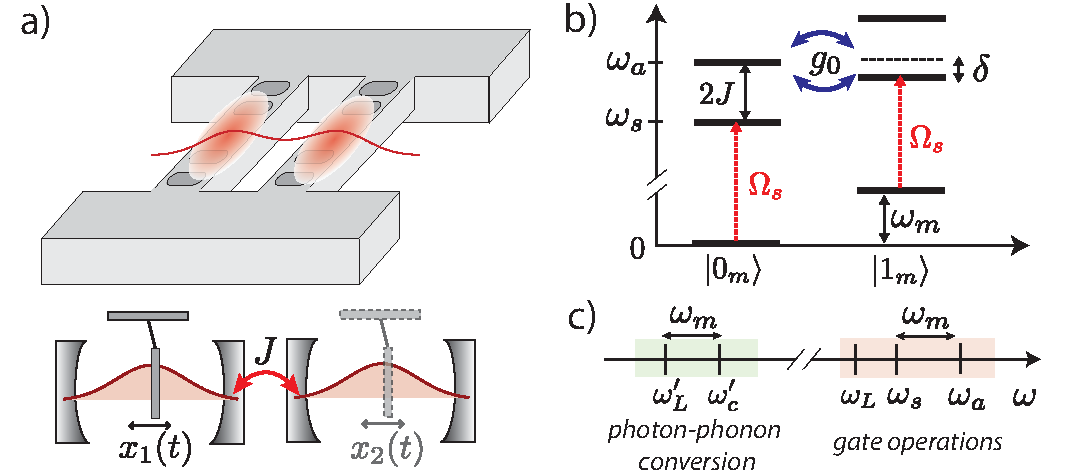
\includegraphics[width=0.9\textwidth]{./figs_Stannigel2012/Figure1.pdf}
\caption
[Model of two resonators]
{ a) Setup of two tunnel-coupled OM crystal cavities (see
Ref.~\cite{Eichenfield2009,Chan2011} for more details).  b) Level
diagram showing the lowest mechanical and optical excitations in a two mode OMS.
Resonant coupling $(\delta=0)$ occurs when the tunnel splitting $2J$ between the
optical modes is comparable to the mechanical frequency $\omega_m$. c) Different
sets of strongly and weakly coupled optical modes and control laser fields can
be used for nonlinear interactions $(\omega_{s},\omega_{a},\omega_L)$ and purely
linear photon storage and retrieval operations
$(\omega_c^\prime,\omega_L^\prime)$.
}
\label{fig:Setup}
\end{center} 
\end{figure}


\section{Model} 

We consider a setup of two tunnel-coupled
OMSs~\cite{Miao2009,Grudinin2010,Dobrindt2010,Safavi-Naeini2011a,Cheung2011}
as schematically shown in Fig.~\ref{fig:Setup}, focusing on the OM crystal
design~\cite{Eichenfield2009,Chan2011} as a specific example.
Each OMS $i=1,2$ is represented by an optical mode of frequency $\omega_c$ and a
bosonic operator $c_{i}$, which is coupled via optical gradient forces to the
motion of an isolated mechanical mode $b_i$ with vibrational frequency
$\omega^i_m$.  The Hamiltonian for this system is $(\hbar=1)$
\begin{equation}\label{eq:H}
\begin{split}
H= &\sum_{i=1,2} \omega_m^i b_i^\dag b_i +  \omega_c c_i^\dag c_i + g_0 c_i^\dag
c_i (b_i+ b_i^\dag) \\
&- J (c_1^\dag c_{2} + c_{1} c_{2}^\dag) +   \sum_{i=1,2}  \Omega_i ( c_i 
e^{i\omega_L t} + �{\rm H.c.}),
\end{split}\end{equation}
where $J$ is the tunneling amplitude between the optical modes and $g_0$ denotes
the single-photon OM coupling; $\Omega_i$ are the local amplitudes of external
control laser fields of frequency $\omega_L$.  Below we also consider an
additional set of cavity modes and driving fields with frequencies
$\omega_c^\prime $ and  $\omega_L^\prime$, respectively.
As indicated in Fig.~\ref{fig:Setup}(c), we assume these modes to be separated
in frequency and used for cooling the mechanical 
modes~\cite{WilsonRaePRL2007, MarquardtPRL2007}, and linear photon storage and
retrieval operations~\cite{Fiore2011, Verhagen2011, Zhang2003, Akram2010} only. 

Apart from the coherent dynamics described by Eq.~\eqref{eq:H}, we include
dissipation through cavity decay and mechanical damping and model the evolution
of the system density operator $\rho$ by a master equation (ME)
\begin{equation}\label{eq:ME}
\begin{split}
\dot \rho = &-i[H,\rho] + \sum_{i}  \kappa \mathcal{D}[c_i] \rho +
\mathcal{L}_\gamma \rho, \\
\end{split} 
\end{equation}
where  $\mathcal{D}[c]\rho=2c\rho c^\dag-\{c^\dag c, \rho\}_+ $, and
$\mathcal{L}_\gamma =\sum_i \frac{\gamma}{2}  (N_{\rm th}+1)   \mathcal{D}[b_i]
+ \frac{\gamma}{2}  N_{\rm th}  \mathcal{D}[b_i^\dag]$.
Here,  $\kappa$ is the optical field decay rate, $\gamma=\omega_m/Q$ the
mechanical damping rate for a quality factor $Q$ and $N_{\rm th}=(e^{\hbar
\omega_m/k_BT}-1)^{-1}$ the mechanical equilibrium occupation number for
temperature $T$. Below we identify $\Gamma_m=\frac{\gamma}{2}(3N_{\rm
th}+\frac{1}{2})$ as the characteristic decoherence rate for mechanical qubit
states\footnote{$\Gamma_m$ corresponds to the initial decoherence rate of a
phonon superposition $(|0_m\rangle+|1_m\rangle)/\sqrt{2}$.}.
\begin{figure}
\begin{center}
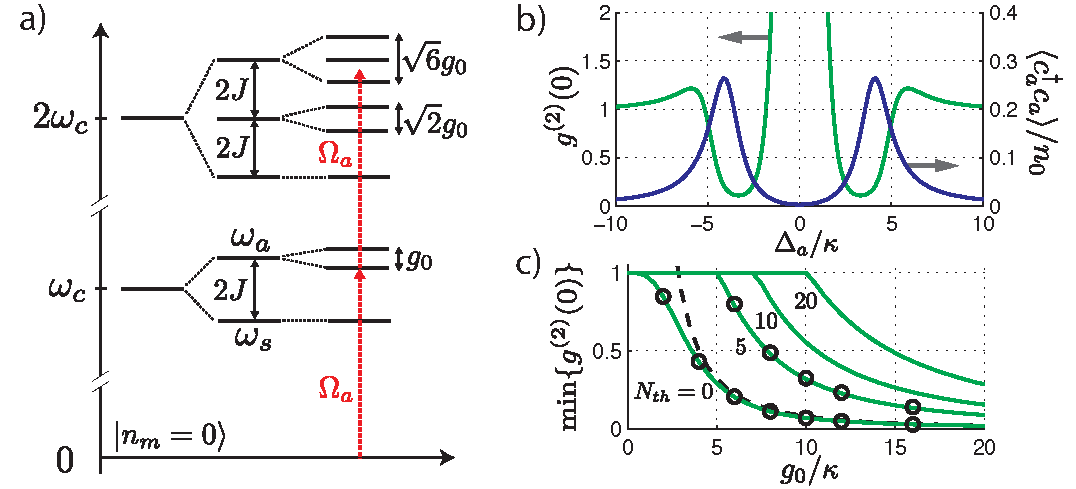
\includegraphics[width=1\textwidth]{./figs_Stannigel2012/Figure2.pdf}
\caption
[Behavior of the coupled system]
{a) Energy level diagram of a resonantly coupled OMS,
$\delta=2J-\omega_m=0$, and for a single mechanical mode in the ground state. b)
Excitation spectrum and $g^{(2)}(0)$ for a weak coherent field exciting the
$c_a$ mode, where $g_0/\kappa=8$ and $n_0=\Omega^2_a/\kappa^2$.  c) Minimal
value of $g^{(2)}(0)$  as a function of the OM coupling strength $g_0$ and for
different values of $N_{\rm th}$. The analytical results (solid lines) given in
the text are in good agreement with exact numerics (circles). The dashed line
shows the asymptotic scaling $\sim 8\kappa^2/g_0^2$ at zero temperature.}
\label{fig:ResonantLevels}
\end{center} 
\end{figure}



\section{Resonant strong-coupling optomechanics}
 
We focus on the strong coupling regime $\omega_m,g_0\gg \kappa,\Gamma_m$,  and
our main goal is to show how the multimode OMS described by Eq.~\eqref{eq:H} can
be used for implementing controlled interactions between qubits encoded in
photonic or phononic degrees of freedom.  To illustrate this we first consider a
single mechanical resonator, $b\equiv b_1$, $\omega_m\equiv \omega_m^1$. We
introduce symmetric and antisymmetric optical modes $c_{s,a}=  \left( c_1 \pm
c_2\right)/\sqrt{2}$ with eigenfrequencies $\omega_{s,a}$ split by $2J$.
Further, we assume that $\omega_m\sim 2J \gg g_0,\kappa, |\delta|$, where
$\delta=2J-\omega_m$  (see Fig.~\ref{fig:Setup}(b)). This condition can be
achieved in nanoscale OMSs where $\omega_m\sim $
GHz~\cite{Eichenfield2009,Chan2011,Carmon2007,Ding2011} and a
matching tunnel splitting can be designed by appropriately adjusting the spacing
between the cavities~\cite{Eichenfield2009,Grudinin2010}. In this
regime we can make a rotating wave approximation with respect to the large
frequency scale $\omega_m \sim 2J$ and after changing into a frame rotating with
$\omega_L$ we obtain~\cite{Grudinin2010}
\begin{equation}\label{eq:HRWA}
H= - \Delta_s c_s^\dag c_s - \Delta_a  c_a^\dag c_a   + \omega_m b^\dag b 
+ \frac{g_0}{2} (c_a c_s^\dag b^\dag +    c_a^\dag c_s  b)+ H_\Omega(t).
\end{equation}
Here $ \Delta_{s,a}= \omega_L - \omega_{s,a}$ are the detunings of the driving
field from the $c_s$ and $c_a$ mode, respectively, and
$H_\Omega(t)=\sum_{\eta=s,a} \left(\Omega_\eta(t) c_\eta + {\rm H.c.}\right)$
accounts for the external driving fields with slowly varying amplitudes
$\Omega_{s,a}(t)=(\Omega_1(t)\pm\Omega_2(t))/\sqrt{2}$.

The two-mode OM coupling in Eq.~\eqref{eq:HRWA} describes  photon transitions
between the energetically higher mode $c_a$ to the lower mode $c_s$, while
simultaneously absorbing or emitting a phonon.  For
$(\Delta_s-\Delta_a-\omega_m)=\delta=0$, this leads to a resonant interaction
between states $|n_a,n_s,n_m\rangle$ and $|n_a-1,n_s+1,n_m+1\rangle$, where
$n_a$, $n_s$ and $n_m$ label the occupation numbers of the two optical modes and
the mechanical mode, respectively.  In analogy to atomic cavity quantum
electrodynamics (QED)~\cite{CavityQEDReview}, the nonlinear scaling of the
corresponding transition amplitudes $\frac{g_0}{2} \sqrt{n_a (n_s+1) (n_m+1)}$
results in an anharmonic level diagram as shown in
Fig.~\ref{fig:ResonantLevels}(a).  If $g_0$ exceeds the cavity linewidth
$\kappa$, one and two photon transitions can be spectrally resolved, indicating
the onset of strong single-photon nonlinearities.


\section{An OM single-photon source}
 
As a potential first application of the nonlinear OM interaction we discuss the
use of the OMS as a single-photon source, which is characterized by a vanishing
equal time two-photon correlation function $g^{(2)}(0)$.  In
Fig.~\ref{fig:ResonantLevels}(b) we plot the excitation spectrum $\langle
c_a^\dag c_a \rangle$ and $g^{(2)}(0)=\langle c_a^\dag c_a^\dag c_a
c_a\rangle/\langle c_a^\dag c_a\rangle^2$,  for the case where only the $c_a$
mode is weakly driven. Around the single-photon resonances $\Delta_a=\pm g_0/2$
we observe strong anti-bunching $g^{(2)}(0)<1$ as a clear signature of
non-classical  photon statistics. To quantify this effect we assume that
$\Gamma_m \ll\kappa$, which allows us to treat subspaces connected to different
$|n_m\rangle$ separately.  For weak driving fields $\Omega_a\ll\kappa$, the
system dynamics can then be restricted to the  six states $ |0_a,0_s,
n_m\rangle, |1_a,0_s, n_m\rangle,|0_a,1_s, n_m+1\rangle,|2_a,0_s, n_m\rangle,
|1_a,1_s, n_m+1\rangle,|0_a,2_s, n_m+2\rangle$ and  we calculate the relevant
occupation probabilities $p_{1,0,n_m}$ and  $p_{2,0,n_m}$ to leading order in
$\Omega_a$~\cite{Carmichael1991}.
We obtain
\begin{equation}
p_{1,0,n}=\abs{ \frac{4\Omega_a d}{ X_n}}^2, \qquad p_{2,0,n} = 8 \abs{
\frac{\Omega_a^2 (8 d^2 - g_0^2)}{( X_n (2X_n -g_0^2))}}^2,
\end{equation}
where $d = \Delta_a - i\kappa$ and $X_n=d^2-g_0^2(n+1)$. By taking the
appropriate thermal averages, $\ev{n_a} = \sum_n \zeta_n p_{1,0,n}$ and
$g^{(2)}(0)  = 2 \sum_n \zeta_n p_{2,0,n}/\ev{n_a}^2$, where
$\zeta_n=(1-e^{-\beta \hbar \omega_m})e^{-\beta \hbar \omega_m n}$ and
$\beta^{-1}=k_B T$, the two photon correlation function can be evaluated for
arbitrary temperatures $T$.

In Fig.~\ref{fig:ResonantLevels}(c) we plot the minimal value of $g^{(2)}(0)$ as
a function of the coupling strength $g_0$ and for different $N_{\rm th}$.
As the OM coupling increases we find that for $T=0$ the minimum of the
correlation function scales as $\textrm{min}_{\Delta_a}\{g^{(2)}(0)\}\simeq 8
\kappa^2/g_0^2$. This demonstrates an improved scaling over off-resonant photon
blockade effects in single-mode OMSs, where for large $\omega_m$ only a small
reduction $g^{(2)}(0)\simeq 1-g_0^2 /(\kappa \omega_m)$ can be
obtained~\cite{Rabl2011}. Since the positions of the single and two-photon
resonances depend explicitly on the mechanical state $|n_m\rangle$,  finite
temperature degrades the quality of the single-photon source.  Nevertheless,
with increasing coupling strength the anti-bunching effect becomes surprisingly
robust and when combined with cooling cycles to achieve $\langle n_m\rangle \sim
1$~\cite{Chan2011}, allows the operation of OM single-photon sources even
at environmental temperatures of a few Kelvin.
\begin{figure}
\begin{center}
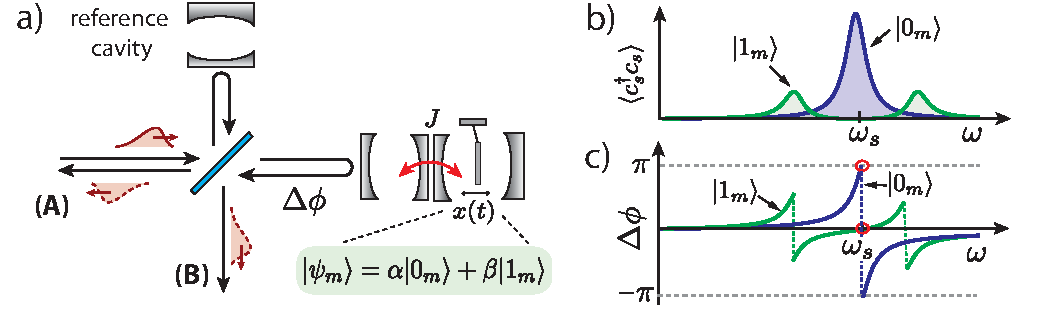
\includegraphics[width=1\textwidth]{./figs_Stannigel2012/Figure3.pdf}
\caption
[A single-phonon single-photon transistor]
{a) An incoming
photon in port (A) passes through the interferometric setup and leaves through
port (A) or (B), depending on the phase shift $\Delta \phi$ acquired upon
reflection from the two-mode OMS.   b), c) For a mechanical system in state
$|0_m\rangle$, the OMS exhibits a single resonance at $\omega_s$ $(\Delta
\phi=\pi$), while for state $|1_m\rangle$  the resonance splits by $g_0\gg
\kappa $ and the photon does not enter the cavity $(\Delta \phi=0)$.  }
\label{fig:SinglePhononTransistor}
\end{center} 
\end{figure}

\section{Single-phonon single-photon transistor}  
Given the ability to generate single photons,
Fig.~\ref{fig:SinglePhononTransistor} illustrates a basic scheme for using the
same resonant OMS to implement a two-qubit gate~\cite{DuanPRL2004}. First, we
assume that the state of a control photon is mapped onto a mechanical
superposition state  $\alpha|0_m\rangle+\beta |1_m\rangle$.
This can be achieved with conventional cooling followed by photon-phonon
conversion techniques using linearized OM interactions with an auxiliary mode
$\omega_c^\prime$ (see Fig.~\ref{fig:Setup}(c)). Next, a single target photon of
central frequency $\sim \omega_s$ is sent through the interferometric setup as
described in Fig.~\ref{fig:SinglePhononTransistor}.
If the mechanical mode is in the state $|0_m\rangle$,  the incoming photon
couples to a single resonant state $|0_a,1_s,0_m\rangle$ (see
Fig.~\ref{fig:Setup}(b)), such that it enters the cavity and picks up a phase
before being reflected.  Instead, if the mechanical resonator is in the state 
$|1_m\rangle$,  the resonant coupling between $|0_a,1_s,1_m\rangle$ and
$|1_a,0_s,0_m\rangle$ splits the cavity resonance, and for $g_0>\kappa$ the
photon is reflected without a phase shift.
Under ideal conditions,  the final result is an entangled state
\begin{equation}\label{eq:Entangled}
|\psi\rangle = \alpha | 0_m, 1_A,0_B\rangle + \beta | 1_m, 0_A,1_B\rangle,
\end{equation}
where $A$ and $B$ are the two ports of the interferometer. This state can be
converted back into an entangled state between the initial control and target
photon.

Assuming that the storage and retrieval of the control photon can be achieved
with high fidelity, the error for producing the entangled
state~\eqref{eq:Entangled} with $\alpha=\beta=1/\sqrt{2}$ is approximately given
by
\begin{equation}\label{eq:Error}
\epsilon  \approx  \frac{4\kappa^2}{g_0^2}+  \frac{1}{(\tau_p \kappa)^{2}}+ 
\tau_p \Gamma_m,
\end{equation} 
where  $\tau_p$ is the duration of the single-photon pulse. The individual
contributions in Eq.~\eqref{eq:Error} arise from an imperfect photon reflection,
the finite spectral width of the photon pulse, and mechanical decoherence,
respectively.
A minimal error is achieved for  $\tau_p^{-1}\approx \sqrt[3]{\kappa^2
\Gamma_m}$ where we obtain $\epsilon\approx {\rm  max} \{  4\kappa^2/g_0^2,
\sqrt[3]{\Gamma_m^2 /\kappa^2}\}$.
Assuming an OM crystal device with $\omega_m/(2\pi)=4$ GHz and $Q=10^5$ as
discussed in Ref.~\cite{Chan2011}, but with an improved OM coupling
$g_0/(2\pi)=50$ MHz and a lower  decay rate $\kappa/(2\pi)=5$ MHz, we obtain
gate errors $\epsilon\approx 0.1$ for environmental temperatures around
$T\approx 100$ mK.




\section{Phonon-phonon interactions}
  
Finally, we consider the possibility to perform a 
controlled gate operation between two qubits stored
in long-lived mechanical modes.
Our approach is depicted 
in Fig.~\ref{fig:PhononQuantumGate}(a), 
and combines the long coherence times of an OM 
quantum memory~\cite{Fiore2011,Verhagen2011,Zhang2003,Akram2010} 
with the practical utility of exploiting interactions 
between stationary phononic qubits.
We focus on the limit $\Gamma_m\ll \kappa$, 
and assume that optical (e.g. `path encoded') 
qubits are first mapped onto long-lived states $|0_m\rangle$ 
and $|1_m\rangle$ of two or more mechanical modes.
The OM coupling is then employed to generate 
nonlinear interactions between the phonons only.  
\begin{figure}
\begin{center}
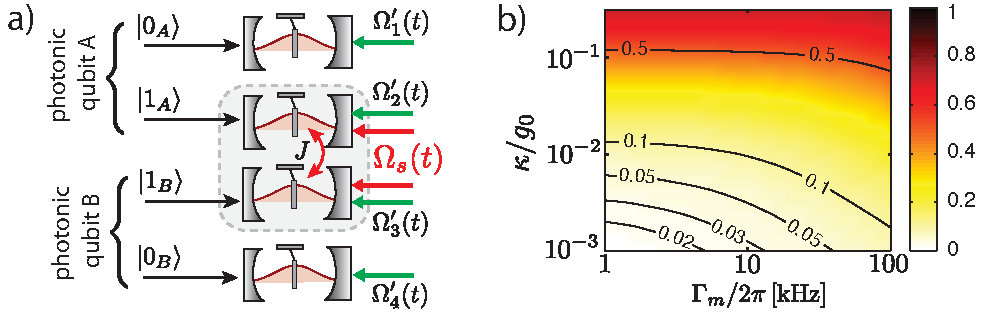
\includegraphics[width=1\textwidth]{./figs_Stannigel2012/Figure4.pdf}
\caption
[Controlled phase gate]
{a) OM quantum memory, where `path-encoded' photonic
qubits are stored in long-lived mechanical states using tunable linearized OM
interactions $\sim\Omega^\prime_i(t)$. Deterministic gate operation between
stationary qubits are implemented by a controlled phonon-phonon interaction
$\sim\Omega_s(t)$ as described in the text. b) The total error $\epsilon_g$ for
implementing a controlled phase gate between two phononic qubits is minimized
with respect to $\Delta_s$ and plotted as a function of $\kappa$ and $\Gamma_m$
(see text). The parameters for this plot are $g_0/(2\pi)=50$ MHz,
$\gamma/(2\pi)=4$ kHz, $\alpha=1$ and $g_0/\delta=1/3$.
}
\label{fig:PhononQuantumGate}
\end{center} 
\end{figure}


We consider nonlinear interactions between
two mechanical modes $b_1$ and $b_2$ described
by Eq.~\eqref{eq:H}, detuned from resonance such that
$g_0< |(2J-\omega_m^i)|$ and direct transitions between  
photons and phonons are suppressed. 
To obtain the effective phonon-phonon interactions,
we first diagonalize
$H$ to second order in $\xi_i = g_0/(2J-\omega_m^i)$
with the transformation
$H\rightarrow e^{iS}He^{-iS}$, 
where 
$S=\frac{i}{2} (c_s^\dag c_a (\xi_1b_1^\dag-\xi_2b_2^\dag) -{\rm H.c.})$.
This yields
 $H= H_0 +H_g+H_\Omega(t)$, where $H_0=  - \Delta_s c_s^\dag c_s - \Delta_a 
 c_a^\dag c_a   + \sum_i \omega^i_m b_i^\dag b_i$,
\begin{equation}\label{eq:Hoff}
	H_g= \frac{g_0}{4} \left[ (c_s^\dag c_s\!+\!1)c^\dag_a c_a (\xi_1\!+\!\xi_2) 
	+ (c_a^\dag c_a\! -\!	c_s^\dag c_s) \mathcal{N}_b \right],
\end{equation}
and we have neglected small corrections to the driving Hamiltonian
$H_\Omega(t)$.
The phonon operator in Eq.~\eqref{eq:Hoff} is given by $\mathcal{N}_b= \xi_1
b_1^\dag b_1+\xi_2 b_2^\dag b_2 - (\xi_1+\xi_2)(b_1^\dag b_2+ b_2^\dag b_1)/2$.
For simplicity we focus on symmetric detuning, $\omega_m^{1,2} = 2J\mp \delta$,
where $\mathcal{N}_b=\frac{g_0}{\delta}(b_1^\dag b_1-b_2^\dag b_2)$.
The  transformation also modifies the dissipative terms in the
Eq.~\eqref{eq:ME}; most importantly, we find an optically-induced decay channel
for the mechanical modes, $\mathcal{L}_\gamma\rightarrow \mathcal{L}_\gamma +
\kappa g^2_0/(4\delta^2) \mathcal{D}[c_s (b_1+b_2)]$.

We assume that only the $c_s$ mode is weakly 
driven by a slowly-varying control field $\Omega_s(t)$. 
In this case the $c_a$ mode remains unpopulated and 
we neglect it. 
Next, we shift the driven mode, $c_s\rightarrow \alpha + c_s$, 
by the classical amplitude $\alpha$,
yielding an effective ME  for $c_s$, $b_1$ and $b_2$.
Finally, we adiabatically eliminate the $c_s$ mode, valid in the
limit $|\alpha|\sim \mathcal{O}(1)$ and $(g_0^2|\alpha|/4\delta)\ll
|\Delta_s+i\kappa|$,
to obtain an effective ME for the mechanical modes (see Appendix
\ref{app:Stannigel2012} for more details), 
\begin{equation}\label{eq:Effective}
\begin{split}
\dot \rho_m =& -i[H_m + \Lambda (b_1^\dag b_1-b_2^\dag b_2)^2 �, \rho_m ] 
+\mathcal{L}_\gamma \rho_m\\
&+ \Gamma_\phi \mathcal{D}[(b_1^\dag b_1-b_2^\dag b_2)]\rho_m   + 
\frac{\gamma^\prime}{2} \sum_i   \mathcal{D}[b_i]\rho_m.
\end{split} 
\end{equation}
Here, $\gamma^\prime=\kappa |\alpha|^2 g_0^2/(2\delta^2)$, and the phonon-phonon
interaction and the phonon dephasing rate are given by
\begin{equation}
\Lambda=\frac{g_{0}^{4}|\alpha|^2  \Delta_{s}}{16 \delta^2
(\Delta_{s}^{2}+\kappa^{2})},\qquad \Gamma_\phi= \frac{g_{0}^{4}|\alpha|^2 
\kappa}{16\delta^2(\Delta_{s}^{2}+\kappa^{2})}.
\end{equation}
The effective Hamiltonian in Eq.~\eqref{eq:Effective} describes 
a phonon nonlinearity with a tunable strength $\Lambda(t)\sim |\alpha(t)|^2$. 
The relevant cross-coupling is given by 
\begin{equation}\label{eq:Heff}
H_{\rm int} \simeq 2 \Lambda b_1^\dag b_1  b_2^\dag b_2,
\end{equation}
and when acting for a time $t_g=\pi/(2\Lambda)$, this Hamiltonian implements a
controlled-phase gate between two qubits encoded in states $|0_m\rangle$ and
$|1_m\rangle$.
During this time, phonons experience intrinsic and optically-induced decoherence
as seen in Eq.~\eqref{eq:Effective}.
In Fig.~\ref{fig:PhononQuantumGate}, we plot the
resulting gate error $\epsilon_g=1-\langle\psi_0|\rho_m(t_g)|\psi_0\rangle$  
for an initial state
$|\psi_0\rangle=\frac{1}{2}(|0_m\rangle+|1_m\rangle)^{\otimes2}$
optimized with respect to $\Delta_s$.
Using the total decoherence rate of this state, 
$\Gamma_{\rm decoh}= 2\Gamma_m+ \Gamma_\phi+ \gamma^\prime/2$, 
we find that  $\epsilon_g\propto\Gamma_{\rm decoh}/\Lambda$ 
is minimized for $|\Delta_s|\simeq g_0/2$, where $\epsilon_g\propto
4(\kappa/g_0)$.
While this scaling with $g_0$ is weaker than for a gate based on photon
reflection (see Eq.~\eqref{eq:Error}), the ability to perform a gate between
stationary qubits represents an important advantage of this approach.

 
\section{Conclusions} 

We have described single-photon and single-phonon nonlinear effects in strongly
coupled multimode OMSs. We have shown how induced nonlinearities on or near
resonance can be used for controlled quantum gate operations between flying
optical or stationary phononic qubits. Our results provide a realistic route
towards the quantum nonlinear regime of OMSs, and a framework for future OM
information processing applications.

 
% Chapter 4: 
\chapter{Heralded Quantum Gates with Integrated Error Detection in Optical Cavities}
\label{ch:Borregaard2015a}
%%%%%%%%%%%%%%%%%%%%%%%%%%%%%%%%%%%%%%%%%%%%%%%%

\section{Introduction}
From \cite{Borregaard2015a}

% Chapter 5:          
\chapter{Long-distance entanglement distribution using individual atoms in
optical cavities}
\label{ch:Borregaard2015b}
%%%%%%%%%%%%%%%%%%%%%%%%%%%%%%%%%%%%%%%%%%%%%%%%
 
\section{Introduction}
From \cite{Borregaard2015b}

% Chapter 6:  
\chapter{Heisenberg-Limited Atom Clocks Based on Entangled Qubits}
\label{ch:Kessler2014}
% From \cite{Kessler2014}
%%%%%%%%%%%%%%%%%%%%%%%%%%%%%%%%%%%%%%%%%%%%%%%%

%%%%%%%%%%%%%%%%%%%%%%%%%%%%%%%%%%%%%%%%%%%%%%%%%%%%%%%%%%%%%%%%%%%%%%%%%%%%%%%%%%5
%%%%%%%%%%%%%%%%%%%%%%%%%%%%%%%%%%%%%%%%%%%%%%%%%%%%%%%%%%%%%%%%%%%%%%%%%%%%%%%%%%5
\section{Introduction}
%%%%%%%%%%%%%%%%%%%%%%%%%%%%%%%%%%%%%%%%%%%%%%%%%%%%%%%%%%%%%%%%%%%%%%%%%%%%%%%%%%5
%%%%%%%%%%%%%%%%%%%%%%%%%%%%%%%%%%%%%%%%%%%%%%%%%%%%%%%%%%%%%%%%%%%%%%%%%%%%%%%%%%5
Currently, atomic clocks based on optical transitions achieve the most
precise \cite{Nicholson2012, Bloom2013, Lemke2009} and accurate \cite{Chou2010,
Bloom2013} frequency references.
Additionally, the development of optical frequency combs
\cite{Eckstein1978, Reichert2000, Jones2000, Ye2003} -- establishing a coherent
link between the optical and radio frequencies -- enabled the application
of optical frequency standards to a wide range of scientific and technological
fields including astronomy, molecular spectroscopy and global
positioning systems (GPS).

% The improvement of frequency standards using quantum resources, such as
% entanglement, has attracted wide attention in recent years \cite{Buzek1999,
% Andre2004, Rosenband2012, Rosenband2012_numerical}.

The improvement of frequency standards using quantum resources, such as
entanglement \cite{Buzek1999, Andre2004,LouchetChauvet:2010fs,Rosenband2012_numerical,
Borregaard2013_nearHeisenberg},
%, as well as
%schemes consiting of multi-layered interrogation and feedback
%\cite{Rosenband2013, Borregaard2013} 
has been actively explored in recent years. While clock protocols
based on uncorrelated atoms at best achieve a stability scaling
$\propto1/\sqrt{N}$, where $N$ is the number of atoms -- a
scaling commonly known as the standard quantum limit (SQL) \cite{Caves1980} --
the use of entangled resources, in principle, allows one to surpass this limit.
However, a characterization of the improvement obtainable by using entanglement
 requires a detailed investigation of the decoherence present in the system.
 Previous studies have focused on two kind of noise sources: i) single particle
 decoherence resulting from the interaction of the atoms with the environment
 and ii) frequency fluctuations in the laser used to excite the clock transition
 [in the following also referred to as local oscillator (LO)].
  It is well known that fully entangled states (e.g.,
  Greenberger-Horne-Zeilinger (GHZ) states) allow for improved spectroscopic sensitivity, but in the same way
 that these states benefit from their increased sensitivity in the laser
 interrogation, they are generically prone to various types of noise sources
 canceling any quantum gain. It has therefore been long believed that such
 states fail to increase clock stability regardless of the noise model being used
 \cite{Bollinger1996, Wineland1998, Rosenband2012_numerical,Huelga1997}. On the other hand, it has been shown that
for clocks with local oscillator noise limited stability, the use of
moderately squeezed atomic states can yield a modest improvement over the SQL
\cite{Andre2004,LouchetChauvet:2010fs}.
 A recent study demonstrated further that, in principle, highly squeezed states
could achieve Heisenberg-limited stability (i.e., a $1/N$ scaling
with the available resources representing the ultimate limit allowed by the laws
of quantum mechanics \cite{Giovanetti2011}) using a complex adaptive
measurement scheme \cite{Borregaard2013_nearHeisenberg}.
 At the same time, it has been shown that the single particle
 decoherence-limited regime can be reached for long averaging time at
a logarithmic cost in $N$ by interrogating uncorrelated atomic
ensembles for suitably chosen times \cite{Rosenband2013, Borregaard2013}.

In this Letter, we  introduce a protocol involving groups of sequentially larger
GHZ states to estimate local oscillator deviations from the atomic reference in
a manner reminiscent of the phase estimation algorithm \cite{Nielsen_Chuang}.
Furthermore, we unify previous treatments of decoherence for atomic clocks 
and incorporate previous proposals involving uncorrelated atoms to
effectively narrow the LO linewidth \cite{Rosenband2013, Borregaard2013} and thereby identify
 ultimate limits to the stability of atomic clocks based on entangled atoms. We find that for LO-noise limited clocks, the
proposed quantum protocol is found to be nearly optimal, realizing the
Heisenberg limit of clock stability up to a logarithmic correction in the
particle number.
Importantly, it reaches the fundamental noise floor  resulting from
individual dephasing of the clock qubits $N$ times faster than the best known
classical schemes, where $N$ is the total number of particles employed.

%In this Letter, we demonstrate that if the dominating noise is LO noise -- as it is the case in modern atomic clocks -- this limitation can be overcome.  
%As the LO fluctuations affect all clock atoms alike, this perfectly correlated noise does not represent a fundamental limitation in the interrogation process, and can be corrected for in a non-adaptive protocol based on multiple GHZ states of varying size, reminiscent of the phase estimation algorithm  \cite{Nielsen_Chuang}. 
%% The procedure is based on the
%% division of the available clock atoms into successively smaller GHZ groups
%% evolving at different phase velocities during the laser interrogation time. Each
%% GHZ group hereby keeps track of the accumulated phase slips of the next
%% ensemble, thus largely eliminating the problem of uncontrolled slips of the
%% laser phase. This allows us to operate a large part of the available resources
%% in a fully entangled state, reaching near-Heisenberg-limited spectroscopy for
%% LO-noise-limited optical clocks,  with an $\mathcal O(\sqrt N/ \mathrmrm{log}(N))$
%% stability improvement over the SQL. 
%We provide the full quantum mechanical
%derivation of this result, 
%% in a feedback analysis, 
%taking into account all relevant noise sources and optimizing over all free
%parameters of the scheme.
%We investigate the limiting factors of atomic clock stability over different
%time scales, and provide a detailed comparison with classical clock protocols.
%The proposed quantum protocol is found to be optimal, realizing the Heisenberg limit of laser stability up to a logarithmic correction in the particle number. It reaches the fundamental noise floor resulting from individual dephasing of the clock qubits $\sim N$ times (with $N$ being the total number of particles employed) faster than the best classical schemes.

The central idea of our approach can be understood as follows.
In modern atomic clocks, the frequency of a LO is locked to an ultra-narrow
 transition of the clock atoms serving as the
frequency reference.
The long-term stability  of such a clock after a given total averaging time
$\tau$ is directly related to the precision by which the accumulated laser phase
relative to the atoms can be determined. To this end, the phase is repeatedly
measured in a standard Ramsey protocol \cite{Ramsey1950}:
Using the LO, the clock qubits are prepared in a superposition of $\ket 1$ and
$\ket 0$, denoting the levels of the clock transition. After the qubits evolve
freely for a time $T$ (Ramsey interrogation time), they are subsequently
measured in an orthogonal basis ($\ket \pm \equiv \ket 1 \pm\ket 0$), which
yields an estimate of the accumulated phase difference between the LO and the
atomic frequency reference.
It is known, that since each of these Ramsey sequences introduces measurement
noise, it is optimal to extend the Ramsey time $T$ 
to its maximum value $T\rightarrow\tau$ \cite{Braunstein:1992bx}.

A single GHZ state consisting of $N$ entangled atoms -- whose state after the
interrogation is $\ket{\mathrm{GHZ}}_T \propto \ket{0}^{\otimes N} + \mathrm{exp}(-i
N\Phi_{\mathrm{LO}}) \ket{1}^{\otimes N}$ -- accumulates the laser phase (denoted
by $\Phi_{LO}$) $N$ times faster than an uncorrelated state, allowin a more precise
phase measurement \cite{Giovanetti2011}. However, fluctuations in the
laser frequency renders the laser phase a
random variable with a probability distribution that grows in width as we
increase  the Ramsey time $T$.
Whenever the laser phase realized in a particular Ramsey cycle induces a full
phase wrap on the state [i.e., the atomic phase $N \Phi_{LO}\notin[-\pi,\pi)$]
a subsequent measurement yields a $2\pi$ error in the estimation. For a single GHZ
state, this accounts for a strict limitation on the maximally allowed Ramsey
time in order  to limit the initial variance of $\Phi_\mathrm{LO}$, and the resulting
laser stability is found to yield no improvement over classical protocols 
\cite{Wineland1998}.

% cause large variations of the phase picked up by the interrogating state in
% the different cycles. Whenever these fluctuations induce a full phase wrap on
% the state [i.e., the atomic phase $N \Phi_{LO}\notin[-\pi,\pi)$] a subsequent
% measurement yields no useful information on the true laser phase due to the
% periodicity of the exponential. For a single GHZ state this accounts for a
% strict limitation on the maximally allowed Ramsey time in order  to limit the
% initial variance of the distribution of $\Phi_\mathrm{LO}$, and thus a resulting
% laser stability that is found to yield no improvement over classical protocols
%  \cite{Wineland1998}.


To address this problem, we use a protocol involving an incoherent version of
the \textit{phase estimation algorithm} \cite{Nielsen_Chuang}, similar to the
one outlined in \cite{Giovannetti2006} but adapted to be applicable also when
the frequency fluctuates and phases exceed $2\pi$. The
phase estimation algorithm has recently been successfully applied experimentally
for global interferometric phase estimation \cite{Higgins2007,Mitchell2005}, and
its use in clock synchronization protocols has been discussed \cite{Burgh2005}.
Here, we demonstrate how the same techniques can be applied to
guarantee optimal laser stability by allowing the Ramsey interrogation
time to be extended to its maximum value.

\begin{figure}
\centering
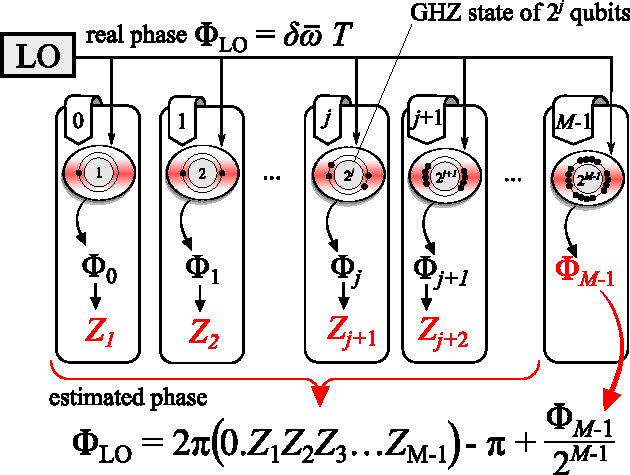
\includegraphics[width=0.8\textwidth]{./figs_Kessler2014/fig2.pdf}
\caption
[GHZ cascade]
{
\label{fig:phase_estimation}
The proposed clock operation scheme employs $M$ different groups of clock atoms
prepared in correlated states of varying size to interrogate the relative phase
$\Phi_\mathrm{LO}$ of the LO field.
A single group $j$ contains $n_0$ independent instances of GHZ-like states, each
entangling $2^j$ qubits, and therefore accumulating a phase $\Phi_j = 2^j
\Phi_\mathrm{LO} \mod [-\pi,\pi]$ during a single cycle. Each group is then used
to measure this phase, which gives a direct estimate on the digit $Z_{j+1}$ in a
binary representation of the LO phase
$(\Phi_\mathrm{LO}+\pi)/2\pi=(0.Z_1Z_2Z_3\hdots)$,
subsequently used to feedback the LO frequency.
}
\end{figure}

Let us assume, for the moment, that the accumulated laser phase after the
interrogation time $T$ lies in the interval $\Phi_\mathrm{LO}\in[-\pi,\pi)$, and
has an exact binary representation $(\Phi_\mathrm{LO}+\pi)/2\pi= \sum_{j=1}^M Z_j/
2^{j}$, with digits $Z_j\in \{0,1\}$ (both conditions will be relaxed below).
One can then readily show that a GHZ state consisting of $2^{M-1}$ atoms picks
up the phase $\Phi_{M-1} = 2^{M-1} \Phi_\mathrm{LO}  ~\mathrm{mod}~ [-\pi,\pi) = \pi
(Z_M-1)$. Thus, by measuring if the phase is $0$ or $\pi$, the last digit of the
laser phase can be determined. However, without
the remaining digits this information is
useless.
In our protocol, these digits are found by an additional, simultaneous
interrogation with successively smaller GHZ states of $2^{M-2},2^{M-3},\hdots$
entangled atoms (see \reffig{fig:phase_estimation}). Each of these states
picks up a phase proportional to its size  $\Phi_{j} = 2^{j}
\Phi_\mathrm{LO}~\mathrm{mod}~ [-\pi,\pi)$, and this
phase gets a contribution of $\pi (Z_j-1)$.
By distinguishing whether the phase is shifted by $\pi$ or not, we can 
determine the value of the bit $Z_j$.
The combined information provides an estimate with an accuracy given by the
largest GHZ state, while the cascade increases the total number of atoms
employed only by a factor of two: $\sum_{j=0}^{M-1} 2^j \approx
2^{M}=2\times2^{M-1}$.

However, in the limit of large averaging times, the assumption
$\Phi_\mathrm{LO}\in [-\pi,\pi)$ is not justified anymore. Here, the optimal
Ramsey time $T\sim\tau$ can attain values that induce phase wraps of the laser
itself, causing the binary representation of the laser phase to contain digits
$Z_j\neq0$ for $j\leq0$, which are inaccessible to the technique discussed
above.
To overcome this, we extend the cascade to
the classical domain, and employ additional groups of {\it uncorrelated}
atoms that interrogate the laser with successively decreasing interrogation times, or
alternatively, using dynamical decoupling techniques \cite{Rosenband2013,
Borregaard2013,ddc}. Each of these ensembles acquires a phase that is
reduced by multiples of two from the laser phase, and thus, following the
arguments from above, allows one to gain information on the digits
$Z_j$ with $j\leq0$.
The information of all digits combined provides the total number of phase wraps,
which in turn yields a Heisenberg-limited estimate of the laser phase.
By this, the protocol effectively eliminates all limitations
arising from the LO noise, and allows the Ramsey time to extend to its optimal
value.

 
% This paper is organized as follows. In Section~\ref{sec:EC} we provide an
% executive summary of the proposed clock operation scheme and the main results of
% our feedback analysis. This Section is self-contained, and can be read without
% consulting the following part of the paper.
% For the interested reader, the subsequent Sections provide the full details of
% our analysis. In Section $\hdots$

% It is a long standing view that GHZ-states cannot increase clock stability due
% to their increased susceptibility to phase slips in the presence of $1/f$-type
% local oscillator noise. \cite{Wineland1998}



%%%%%%%%%%%%%%%%%%%%%%%%%%%%%%%%%%%%%%%%%%%%%%%%%%%%%%%%%%%%%%%%%%%%%%%%%%%%%%%%%%5
%%%%%%%%%%%%%%%%%%%%%%%%%%%%%%%%%%%%%%%%%%%%%%%%%%%%%%%%%%%%%%%%%%%%%%%%%%%%%%%%%%5
\section{Feedback loop}
%%%%%%%%%%%%%%%%%%%%%%%%%%%%%%%%%%%%%%%%%%%%%%%%%%%%%%%%%%%%%%%%%%%%%%%%%%%%%%%%%%5
%%%%%%%%%%%%%%%%%%%%%%%%%%%%%%%%%%%%%%%%%%%%%%%%%%%%%%%%%%%%%%%%%%%%%%%%%%%%%%%%%%5
In the following, we provide a derivation of the above results
combined with feedback analysis that allows us to characterize
the achievable stability of a clock using our protocol. Modern
clocks periodically measure the fluctuating LO frequency $\omega(t)$ against the
frequency standard $\omega_0$ of the clock atoms to
obtain an error signal.
After each Ramsey cycle of duration $T$ [i.e., at times $t_k=kT$
($k=1,2\hdots$)], the measurement data yield
 an estimate of the relative phase, $\Phi_\mathrm{LO}(t_k) =
\int_{t_k-T}^{t_k}\d{t}[\omega(t) - \omega_0]$, accumulated by the LO.
This estimate in turn is used to readjust the frequency of the LO:  $\omega(t_k)
\rightarrow \omega(t_k) - \alpha\Phi^\mathrm{est}_\mathrm{LO}(t_k)/T$, where
$\Phi^\mathrm{est}_\mathrm{LO}(t_k)$ represents a suited estimator of the phase
$\Phi_\mathrm{LO}(t_k)$ \footnote{Alternatively, it is also possible to perform direct phase
feedback.}, and $\alpha < 1$ is an suitably chosen
gain.
%Phase feedback
%is chosen since it performs better in the presence of white noise
%\cite{Bollinger1996}, but one can use frequency
%feedback and achieve the same stability up to a constant factor.

The stability of the actively stabilized LO, after a total averaging time
$\tau$, is characterized by the Allan deviation (ADEV) which is directly
proportional to the measurement uncertainty $\Delta\Phi_\mathrm{LO}(t_k)$ after
each Ramsey cycle (see Appendix \ref{app:Kessler2014}),
\bel
	\label{eq:Allan-variance}
	\sigma_y(\tau) \equiv \frac{1}{\omega_0 \tau}
	\sqrt{\sum_{k = 1}^{\tau/T}\sum_{l = 1}^{\tau/T}
	T^2\ev{\delta\bar\omega_k\delta\bar\omega_l} }
	\approx
	 \frac{1}{\omega_0\sqrt{\tau T}} \Delta\Phi_\mathrm{LO}(T).
%  	 =
% 	\frac{1}{\omega_0^2\tau T} \frac{(\Delta\Phi_{M-1})^2}{D^{2M-2}}
% 	=:
% 	\frac{\gamma}{\omega_0^2 \tau} S^2(\gamma T,D,M,N)  ,
\eel
Here, $\delta\bar\omega_k = \Phi_\mathrm{LO}(t_k)/T$ is the average detuning of the
(stabilized) LO during the $k$th cycle. {%
 To obtain \refeq{eq:Allan-variance}, we use the fact that after the frequency
 feedback the detuning averages become approximately uncorrelated for realistic
 laser spectra, $\ev{\delta\bar\omega_k \delta\bar\omega_l} \approx
 \ev{\delta\bar\omega^2}\delta_{kl}$ \cite{Borregaard2013,
 Andre2005,Bloom2013}}.
%It has been shown that, if the frequency noise spectrum of the free running LO,
%$S_\omega(f)$, is less divergent than $\mathcal{O}(1/f^2)$ as  $f\rightarrow 0$,
%then the low-frequency part of the frequency noise spectrum of the actively
%stabilized LO $S^\mathrm{st}_\omega(f)$ is dominated by white noise originating
%entirely from measurement uncertainties \cite{Borregaard2013, Andre2005}.
%Since realistic laser noise spectra -- being dominated by white and $1/f$-noise
%(electronic flicker noise) \cite{Bishof2013} -- fulfill this condition,
%different Ramsey cycles are independent, and write the covariance as
%$\ev{\delta\bar\omega_k \delta\bar\omega_l} = \ev{\delta\bar\omega^2}\delta_{kl}
%= (\Delta \Phi_\mathrm{LO})^2\delta_{kl}/T^2$, which results in the right hand
 %side of \refeq{eq:Allan-variance}.
Other noise sources (such as the bias of the linear estimator, the Dick effect,
or a sub-optimal gain $\alpha$ \cite{Santarelli1998}) are not fundamental, and
neglected in the following.


%%%%%%%%%%%%%%%%%%%%%%%%%%%%%%%%%%%%%%%%%%%%%%%%%%%%%%%%%%%%%%%%%%%%%%%%%%%%%%%%%%5
%%%%%%%%%%%%%%%%%%%%%%%%%%%%%%%%%%%%%%%%%%%%%%%%%%%%%%%%%%%%%%%%%%%%%%%%%%%%%%%%%%5
\section{Spectroscopic nosies}
%%%%%%%%%%%%%%%%%%%%%%%%%%%%%%%%%%%%%%%%%%%%%%%%%%%%%%%%%%%%%%%%%%%%%%%%%%%%%%%%%%5
%%%%%%%%%%%%%%%%%%%%%%%%%%%%%%%%%%%%%%%%%%%%%%%%%%%%%%%%%%%%%%%%%%%%%%%%%%%%%%%%%%5

For small values of the accumulated Ramsey phase, the ultimate precision by
which this phase can be estimated is determined by the Cram\'{e}r-Rao bound
\cite{Rao1945,Giovanetti2011} which 
links the estimation error to the quantum Fisher information (QFI)
$\Delta\Phi_\mathrm{LO} \sim 1/\sqrt{\mathcal F}$ (for a review, see
\cite{Giovanetti2011}). The QFI, $\mathcal F$, is maximized, e.g., by the use of
GHZ states for which $\mathcal F \sim N^2$.
In clock stabilization, however, the LO frequency fluctuations account for the
fact that the accumulated Ramsey phase is a random variable which can obtain
large values, inherently violating the small phase assumption of the
Cram\'{e}r-Rao bound.
% A phase wrap error occurs whenever $\Phi(t_k)$ falls outside the interval
% $[-\pi,\pi)$ at the end of the $k$th cycle which can not be detected in a
% standard Ramsey measurement.
In particular for a single GHZ states, phase wraps of the atomic phase,
$\Phi(t_k)=N \Phi_\mathrm{LO}(t_k)\notin[-\pi,\pi)$, cannot be detected.
Consequently, the cycle time $T$ has to be
chosen such that the prior distribution of $\Phi(t_k)$ is well localized
within $[-\pi,\pi)$.
This limits the maximally allowed Ramsey time to a value $T_\mathrm{max}
\sim\gamma_\mathrm{LO}^{-1}/N^2$ (see 
Appendix \ref{app:Kessler2014}), where we assumed a white frequency noise
spectrum of the LO, $S_\omega(f) = \gamma_\mathrm{LO}$ (for $1/f$-noise one finds the less stringent
condition $T_\mathrm{max} \sim\gamma_\mathrm{LO}^{-1}/N$). In most cases, this value
lies below the optimal (i.e., maximal) value implied by
\refeq{eq:Allan-variance} $T\sim\tau$, resulting in a laser stability for GHZ
states which shows no improvement over the stability achieved with uncorrelated
atoms \cite{Wineland1998, Rosenband2012_numerical}.

However, unlike the individual particle noise resulting in the finite atom
linewidth $\gamma_\mathrm{ind}$, the LO frequency fluctuations affect all clock
atoms alike, and this \textit{collective noise} does not represent a fundamental
metrological limitation.
Ee can use a cascade of GHZ states of varying size to measure the
$\Phi_\mathrm{LO}$ in a binary representation, as discussed above.
In general, the phase does not have an exact binary representation ending at the
digit $Z_{M}$. We therefore employ $n_0$ duplicates  at each level of the
cascade (as opposed to sequential procedure suggested in \cite{Giovannetti2006})
($n_0 =N/\sum_{j=0}^{M-1} 2^j \approx N/2^M$) to improve the precision.
 In the case where all digits $Z_j$ ($j=1\dots, M-1$) are determined correctly
 according to the relation
\bel
Z_j =
[2(\Phi_{j-1}+\pi) - (\Phi_j + \pi)]/2\pi,
\eel
the last group ($j=M-1$) then yields a Heisenberg-limited estimate of
the LO phase with accuracy $(\Delta\Phi_\mathrm{LO})_\mathrm{pr} =
1/(2^{M-1} \sqrt{n_0}) = 2\sqrt{n_0}/N$.

%%%%%%%%%%%%%%%%%%%%%%%%%%%%%%%%%%%%%%%%%%%%%%%%%%%%%%%%%%%%%%%%%%%%%%%%%%%%%%%%%%5
%%%%%%%%%%%%%%%%%%%%%%%%%%%%%%%%%%%%%%%%%%%%%%%%%%%%%%%%%%%%%%%%%%%%%%%%%%%%%%%%%%5
\subsection{Phase estimation with multiple GHZ groups}
%%%%%%%%%%%%%%%%%%%%%%%%%%%%%%%%%%%%%%%%%%%%%%%%%%%%%%%%%%%%%%%%%%%%%%%%%%%%%%%%%%5
%%%%%%%%%%%%%%%%%%%%%%%%%%%%%%%%%%%%%%%%%%%%%%%%%%%%%%%%%%%%%%%%%%%%%%%%%%%%%%%%%%5
%{\it Cascaded GHZ.}---

%Let us assume for the moment that the prior distribution of the LO phase $\Phi_\mathrm{LO}$ after the
%Ramsey time is localized in $[-\pi,\pi)$ (we will relax this condition below), such that we can write $(\Phi_\mathrm{LO}+\pi)/
%2\pi= \sum_{j=1}^\infty Z_j/ 2^{j}\equiv0.Z_1Z_2Z_3\hdots$

%0.Z_1Z_2Z_3\hdots$. 
%Then we can
%represent the  phase we want to estimate as a binary fraction
%$(\Phi_\mathrm{LO}+\pi)/2\pi= \sum_{j=1}^\infty Z_j/ 2^{j}\equiv
%0.Z_1Z_2Z_3\hdots$, with digits $Z_j\in\{0,1\}$.


%We imagine dividing the $N$ qubits available into $M$ groups
%($j=0,1\dots M-1$), each containing $n_0$ independent instances of  $2^j$ number of
%qubits entangled in a GHZ state, $\ket{\mathbf{1}}_j + i \ket{\mathbf{0}}_j
%\equiv\ket{0}^{\otimes{2^j}} + i\ket{1}^{\otimes{2^j}}$ ($n_0 =
%N/\sum_{j=0}^{M-1} 2^j \approx N/2^M$), as shown in \reffig{fig:phase_estimation}.
 %Subsequently, the LO field is
% (with average detuning $\delta\bar\omega$)
%interrogated by all entangled states simultaneously  in a Ramsey cycle of length
%$T$, using the technique described in \cite{Bollinger1996}.
%After this interrogation the respective GHZ states are given as
%$\ket{\mathbf{1}}_j + i e^{i\Phi_j} \ket{\mathbf{0}}_j $ having accumulated the
%phase 
%\begin{align} \label{eq:EK1}
%\Phi_j =& 2^j \Phi_\mathrm{LO}  ~\mathrm{mod}~ [-\pi,\pi) \\ 
%=&2\pi 
%(0.Z_{j+1} Z_{j+2} Z_{j+3}\hdots)-\pi.
%\end{align}
%The largest group
%$j=M-1$ (i.e., the group with the fastest evolving GHZ states) consequently 
%can estimate $\Phi_{M-1} =2\pi  (0.Z_{M} Z_{M+1} \hdots)-\pi $ with accuracy
%$\Delta\Phi_{M-1} = 1/\sqrt{n_0} $ \cite{Itano1993,fn2}.
%The number of phase slips  $Z_1\hdots Z_{M-1}$ -- necessary to derive an estimate of the laser phase $\Phi_{LO}$ --  subsequently can be measured directly digit by digit from the groups of
%successively smaller GHZ states according to the relation 
%\bel
%Z_j =
%[2(\Phi_{j-1}+\pi) - (\Phi_j + \pi)]/2\pi
%.
%\eel If all digits $Z_j$ are determined correctly this yields a Heisenberg-limited estimate of
%the LO phase with accuracy $(\Delta\Phi_\mathrm{LO})_\mathrm{pr} =
%1/(2^{M-1} \sqrt{n_0}) = 2\sqrt{n_0}/N$, and with a Ramsey time that 
%can exceed the laser noise limit $T_\mathrm{max}$.

However, in general the estimation of the binary digits $Z_j$ is not perfect.
A rounding error occurs whenever $|\Phi_{j-1}^\mathrm{est} - \Phi_{j-1}| > \pi/2$
(where $\Phi_j^\mathrm{est}$ represents a suitable estimator derived from the $n_0$
measurement outcomes), leading to the wrong $Z_j$, and a variance contribution
of $(2\pi 2^{-j})^2$ for $\Phi_\mathrm{LO}$.
We can approximate their total
variance contribution with the sum
 $ 	(\Delta\Phi_\mathrm{LO})^2_\mathrm{re} = P_\mathrm{re}\sum_{j=1}^{M-1}
 	(2\pi 2^{-j})^2
%  	\frac{D}{\pi}\exp\left[-\frac{\pi^2}{D^2}n_0\right] 
%  	\approx 4\pi D^{2M-3}
%  	\exp\left[-\frac{\pi^2}{D^2}n_0\right].
 $, where 
$P_\mathrm{re} = 2\intop_{\pi/2}^{\infty}\d{\phi}
\rho(\phi)$, 
% \bel
% 	\label{eq:p_re}
% 	p_\mathrm{rounding error} = 2\intop_{\pi/2}^{\infty}\d{y} \rho(y) <
% 	2\intop_{\pi/2}^{\infty}\d{y} n_0 e^{-n_0y^2} 
% 	=
% 	\frac{2}{\pi}\exp\left[-\frac{\pi^2}{2^2}n_0\right] \left(1 +
% 	\mathcal{O}\left(\frac{2}{\pi}\right)\right), \qquad \forall j,
% \eel
and $\rho(\phi)$ is the Gaussian probability distribution of the error
$\Phi_j^\mathrm{est} - \Phi_j$ with a width proportional to $1/\sqrt n_0$  
(see Appendix \ref{app:Kessler2014}).
Consequently, rounding errors can be exponentially suppressed by choosing a
sufficiently large value for $n_0$. The total
measurement uncertainty of this estimation scheme is thus
$(\Delta\Phi_\mathrm{LO})^2 = (\Delta\Phi_\mathrm{LO})_\mathrm{pr}^2
+(\Delta\Phi_\mathrm{LO})_\mathrm{re}^2$.
In Appendix \ref{app:Kessler2014}, we show that the optimal allocation of
resources is achieved for the choice $n_{0}^{\mathrm{opt}} \sim
\frac{16}{\pi^2}\log\left(N\right)$, for which rounding errors are negligible,
yielding the total measurement accuracy
 \bel
 \label{eq:M}
\Delta\Phi_\mathrm{LO} \approx (\Delta\Phi_\mathrm{LO})_\mathrm{pr} =
\frac{8}{\pi}\sqrt{\mathrm{log}(N)}/N.
\eel This measurement precision obtains the Heisenberg limit (up to a
logarithmic correction resulting from the cost to suppress rounding errors)
despite it being applicable to a general (typically large) phase.

% \bel
% \tilde\Phi_j = (\Phi_j \mod [-\pi,\pi])= (D^j T\delta\bar\omega \mod
% [-\pi,\pi]),\qquad\qquad \Delta\tilde\Phi_j =
% \frac{1}{\sqrt{n_0}} \quad \forall j\qquad\mathrm{(from MLE)}
% \eel
% where $T$ is the free evolution time (See \reffig{fig:phase_estimation}).
% Its
% uncertainty is a good approximation
% % (strictly speaking, an upper bound) 
% of the uncertainty of $\Phi_\mathrm{LO}$, $\Delta\Phi_\mathrm{LO} =
% \Delta\Phi_{M-1}/D^{M-1}$.
% % \bel
% % 	\Delta\Phi_\mathrm{LO} = \frac{\Delta\Phi_{M-1}}{D^{M-1}}.
% % \eel
% Unfortunately, 

%Note, that this estimation protocol can be understood as an incoherent
%version of the phase estimation algorithm. However, as compared to previous versions of the latter \cite{Geza} the measurement uncertainty is
%reduced by a factor $ \propto 2^{M/2}/\sqrt{\mathrm{log}(N)}$ enabling the full
%quantum gain of our protocol.

So far we have assumed that $\Phi_\mathrm{LO}\in[-\pi,\pi)$ in each cycle.
However, for realistic laser noise spectra there is always a finite probability
that the LO phase $\Phi_\mathrm{LO}$ lies outside the interval $[-\pi,\pi)$ after
the interrogation time. Such phase wraps of the laser phase itself add to the
final measurement uncertainty in \refeq{eq:M} by the amount
$
	(\Delta\Phi_\mathrm{LO})^2_\mathrm{slip} =  (2\pi)^2P_\mathrm{slip}
$,
where 
$P_\mathrm{slip} = 2\intop_\pi^\infty \d{\phi} \rho_\mathrm{LO}(\phi)$,
% \bel
% 	\label{eq:p_slip}
% 	p_\mathrm{slip} = 2\intop_\pi^\infty \d{y} \rho_\mathrm{LO}(y) = 2\intop_\pi^\infty
% 	\d{y} \frac{1}{\sqrt{2\pi (\gamma T)^2}}
% 	\exp\left[-\frac{y^2}{2(\gamma T)^2}\right] = \sqrt{\frac{2}{\pi}}
% 	\frac{\gamma T}{\pi}\exp\left[-\frac{\pi^2}{2(\gamma T)^2}\right] \left(1
% 	+ \mathcal{O}\left(\frac{\gamma T}{\pi}\right)\right),
% \eel
and $\rho_\mathrm{LO}$ is the Gaussian prior distribution of $\Phi_\mathrm{LO}$.
Its width grows with $ \gamma_\mathrm{LO} T$, which puts a constraint on the
maximally allowed Ramsey time $T
\leq\frac{\pi^2}{4}\gamma_\mathrm{LO}^{-1}[\log(\gamma_\mathrm{LO}\tau N)]^{-1}$,
and thus the achievable ADEV $\sigma_y~(\propto 1/\sqrt T)$
 as we demonstrate in Appendix \ref{app:Kessler2014}.

This, however, does not represent a fundamental limitation as we can
extend the scheme by adding additional classical measurements with a shorter
Ramsey periods to assess the number of phase slips of
the laser phase itself $\hdots Z_{-3}Z_{-2}Z_{-1}Z_0$. As demonstrated in
Appendix \ref{app:Kessler2014}, this allows  extending the Ramsey time by a
factor $k$ adding only a negligible number of atoms $N^{*}\approx
\frac{8}{\pi^2} \log\left(k N^2\right)\log_2(k)\ll N$.
% This procedure can be understood as a classical pre-narrowing of the laser
% linewidth before the application of the quantum protocol.

% Using classical techniques the effective laser linewidth can be pre-narrowed
% before application of the proposed quantum protocol. This is achieved in a
% parallel interrogation with classical ensembles that measure the laser phase
% using varying Ramsey times, or alternatively, by employing dynamical
% decoupling techniques \cite{Rosenband2013, Borregaard2013,ddc}.
 % It allows the extension of the Ramsey time by a factor $k$ at negligible cost
 % in total resources $N^{*}\approx \frac{2}{\pi^2} D^2 \log\left(k
 % N^2\right)\log_D(k)\ll N$.
 % As we demonstrate in the SI, this can be understood as an extension of the
 % cascaded interrogation scheme to the classical domain to assess the binary
 % digits left of the point, $Z_j$ ($j<0$), eliminating the threat of
 % unaccounted phase slips of the laser phase.
 
% The Ramsey time is then only limited by individual noise processes resulting
% in the finite linewidth of the clock atoms $\gamma_\mathrm{ind}$ which put a
% fundamental limit on the allowed Ramsey time
% $T\leq\gamma_\mathrm{ind}^{-1}/2^{M-1}$, inversely proportional to the size of
% the GHZ states in group $M-1$.




%However, also here rounding errors do not represent a fundamental limitation. The necessity of using multiple copies $n_0$ can in principle be avoided by a quantum processing step of the clock atom state prior to the measurement. After the the interrogation time T the total state of the system is given as
%\begin{align}
%\Ket{\Psi} =\frac{1}{2^{M/2}}& \left( \Ket{\mathbf0}_0 + e^{i2^0\Phi_\mathrm{LO}}\Ket{\mathbf{1}}_0\right)\left( \Ket{\mathbf0}_1 + e^{i2^1\Phi_\mathrm{LO}}\Ket{\mathbf{1}}_1\right)\hdots\\
%&\left( \Ket{\mathbf0}_{M-1} + e^{i2^{M-1}\Phi_\mathrm{LO}}\Ket{\mathbf{1}}_{M-1}\right),
%\end{align}
%where we defined the logical qubits $\Ket{\mathbf0}_j = \Ket{0}^{\otimes 2^j}$ ($\Ket{\mathbf1}_j = \Ket{1}^{\otimes 2^j}$), according to the different GHZ groups. In the pathological case that $\phi_\mathrm{LO}$ has an exact $M$ bit binary representation, one readily shows that application of the inverse quantum Fourier transformation $U_\mathrm{QFT}^{-1}$ on the logical qubit state yields
%\bel
%U_\mathrm{QFT}^{-1} \Ket \Psi =\Ket{Z_1Z_2...Z_M},
%\eel
%such that a measurement of the logical qubits directly gives perfect information on $\phi_\mathrm{LO}$. Also in the general case of an arbitrary value of $\phi_\mathrm{LO}$, the measurement of the logical qubits in the computational basis yields an accurate estimate of the LO phase with uncertainty $(\Delta \Phi_\mathrm{LO})^2 \approx 2^{-2(M-1)}$. 

% Here, we note that the exponential dependence with $M$ translates to a
% polynomial dependence of $N$ after optimizing the value of $M$, which is
% then outweighed by the exponential scaling of $P_\mathrm{re}$. As a result, the
% noise from rounding errors is negligible compared to the projection noise at the
% optimal working point. 


%Although, individual atom dephasing affects negligibly the stability in the case
%of uncorrelated atoms, it
%contributes significantly for GHZ states with sufficiently large number of
%entangled atoms. This effect of this dephasing is increased by a factor of
%$2^{M-1}$  on the $j=M-1$ group, compared to the uncorrelated group ($j=0$),
%yielding the variance contribution
%\bel
%	(\Delta\Phi_{M-1})^2_\mathrm{ind} = 2^{M-1}\frac{\gamma_\mathrm{ind}T}{n_0},
%\eel
%where $\gamma_\mathrm{ind}$ is the atomic linewidth. 
% 	\sqrt{\frac{2}{\pi}} \frac{\gamma T}{\pi}\exp\left[-\frac{\pi^2}{2(\gamma
% T)^2}\right].
%The full variance of  $\Phi_{M-1}$ is given as the
%sum, $(\Delta\Phi_{M-1})^2 = (\Delta\Phi_{M-1})^2_\mathrm{pr} +
%(\Delta\Phi_{M-1})^2_\mathrm{re} + (\Delta\Phi_{M-1})^2_\mathrm{slip} +
%(\Delta\Phi_{M-1})^2_\mathrm{ind}$, assuming $P_\mathrm{re}, P_\mathrm{slip} \ll 1$. 
% Finally
% $\mathrm{Var}(\Phi_\mathrm{LO}) = \frac{(\Delta\Phi_{M-1})^2}{D^{2M-2}}$.
% \bel
% 	(\Delta\Phi_{M-1})^2 = ([\Delta\Phi_{M-1}]_\mathrm{pr})^2 +
% 	([\Delta\Phi_{M-1}]_\mathrm{re})^2 + ([\Delta\Phi_{M-1}]_\mathrm{slip})^2.
% \eel


%%%%%%%%%%%%%%%%%%%%%%%%%%%%%%%%%%%%%%%%%%%%%%%%%%%%%%%%%%%%%%%%%%%%%%%%%%%%%%%%%%5
%%%%%%%%%%%%%%%%%%%%%%%%%%%%%%%%%%%%%%%%%%%%%%%%%%%%%%%%%%%%%%%%%%%%%%%%%%%%%%%%%%5
\subsection{Optimization}
%%%%%%%%%%%%%%%%%%%%%%%%%%%%%%%%%%%%%%%%%%%%%%%%%%%%%%%%%%%%%%%%%%%%%%%%%%%%%%%%%%5
%%%%%%%%%%%%%%%%%%%%%%%%%%%%%%%%%%%%%%%%%%%%%%%%%%%%%%%%%%%%%%%%%%%%%%%%%%%%%%%%%%5
With all phase wraps counted correctly, the Ramsey time is only limited by
individual noise processes. The finite linewidth of the atomic clock transition
$\gamma_\mathrm{ind}$ gives rise to the fundamental constraint
$T\leq\gamma_\mathrm{ind}^{-1}/2^{M-1}$.
For averaging times
$\tau\leq\gamma_\mathrm{ind}^{-1}/2^{M-1}$, we can choose $T \approx \tau$, and
using the optimized value for $n_0$ found above the resulting clock stability is
obtained from \refeq{eq:Allan-variance}
\bel
	\label{eq:sigma(1)}
	\sigma_y(\tau)^{(1)} \approx	
	%\frac{1}{\omega_0\tau}
	%\frac{1}{\sqrt{n_{0,\mathrm{opt}}} 2^{M-1}}=
	\frac{2}{\omega_0\tau}
	\frac{\sqrt{n_{0}^{\mathrm{opt}}}}{N} \approx	\frac{8}{\pi\omega_0\tau}
	\frac{\sqrt{\mathrm{log}(N)}}{N}.
\eel
It scales linearly with the averaging time $\tau$, and realizes the Heisenberg
bound of laser stability up to a logarithmic correction. In contrast, in the regime $\tau\geq\gamma_\mathrm{ind}^{-1}/2^{M-1}$, $T$ is limited
by the presence of individual particle noise to a value $T\approx \gamma_\mathrm{ind}^{-1}/2^{M-1}= 2 \gamma_\mathrm{ind}^{-1}n_0/N$, and we find
\bel
	\label{eq:sigma(2)}
	\sigma_y(\tau)^{(2)} \approx
	\frac{1}{\omega_0}  \sqrt{\frac{\gamma_\mathrm{ind}}{\tau N}}.
\eel
\refeq{eq:sigma(2)} represents the fundamental noise floor for laser stability
resulting from quantum metrological bounds in the presence of individual
particle noise \cite{Escher:2011fn}. As we have seen, the proposed protocol
reaches this optimal value rapidly after the averaging time $\tau_0 \sim  
\gamma_\mathrm{ind}^{-1} \mathrm{log}(N)/N$ (cf. \reffig{fig:sigma_tau}),
$N/\mathrm{log}(N)$ times faster than any classical scheme.
In Appendix \ref{app:Kessler2014} we derive the necessary threshold fidelities in
the GHZ state preparation our scheme can tolerate without compromising the stability
in Eqs.~(\ref{eq:sigma(1)}) \& (\ref{eq:sigma(2)}).

\begin{figure}
\centering 
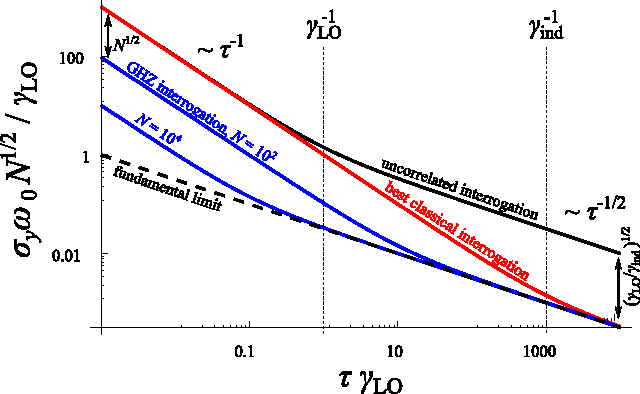
\includegraphics[width=0.9\textwidth]{./figs_Kessler2014/fig1.pdf}
\caption
[Comparison of clock protocols] 
{
\label{fig:sigma_tau}
Allan deviation $\sigma_y$ for different protocols as a function of averaging
time $\tau$, normalized to the standard quantum limit, for $\gamma_\mathrm{LO} /
\gamma_\mathrm{ind} = 10^3$. The solid black line corresponds to the standard scheme using
a single uncorrelated ensemble. It fails to reach the fundamental noise floor
set by the atomic transition linewidth (cf. \refeq{eq:sigma(2)}, broken line).
A more sophisticated classical scheme which uses exponentially increasing Ramsey
times in each cycle \cite{Rosenband2013, Borregaard2013} allows to extend the
regime of linear scaling with $1/\tau$ up to the point where the bound
(\ref{eq:sigma(2)}) is met. In comparison, the proposed cascaded GHZ protocol
(blue solid curves) enables an $\sim N$ times faster convergence. For short
averaging times the stability is enhanced by a factor $\sqrt{N}$ as compared to
classical protocols.
}
\end{figure} 


% 
% , where
% \bel
% 	\label{eq:S^2}
% 	S^2(\gamma T,C) = \frac{1}{\gamma T} C 
% 	+ \sqrt{32\pi}	\exp\left[-\frac{\pi^2}{2(\gamma T)^2}\right],
% \eel
% and
% \bel
% 	\label{eq:C}
% 	C(D,M,N) = \frac{1}{N D^{M-1}} +
% 	\frac{8\pi
% 	N^{1/2}}{D^{\frac{M+1}{2}}}\exp\left[-\frac{\pi^2 N}{2D^{M+1}}\right],
% \eel
% which can be obtain by approximating the
% integrals of the Gaussians with the first term of the asymptotic series,
%  $\int_x^\infty \d{\xi}\exp[-\xi^2/2] = \exp[-x^2/2]\left(1/x +
% \mathcal{O}(x^{-2})\right)$, and assuming $\sum_{j=0}^{M-1}D^j \approx D^{M-1}$.
% % Appendix \ref{sec:Optimization} contains the details of carrying out the
% % optimization.
% 
% The highest stability is achieved for the minimal $S^2$, which can be found by
% direct optimization, which we carry out in three steps.
% First, we find $\gamma T_\mathrm{opt}$ in terms of $C$, by finding the global
% minimum of \refeq{eq:S^2} analytically, in the limit $\gamma T \ll 1$, using the
% general solution of the transcendental equation $x^n = A\exp[-1/x]$ in the case
% of $A\gg 1$ (see Supplementary Materials).
% This yields $\gamma T_\mathrm{opt} =
% \frac{\pi}{\sqrt{2}}\left[\log\frac{8\pi^{3/2}}{C}\right]^{-1/2}$.
% The resulting function $S^2( \gamma T_\mathrm{opt}(C), C)$ is monotonically
% decreasing for $C \ll 1$, which is the relevant region for us.
% In the second step, we find $D_\mathrm{opt}$ in terms of $M$ and $N$ by finding
% the global minimum of \refeq{eq:C} analytically in the limit $N/D^{M+1} \gg 1$,
% using the same technique.
%%%%%%%%%%%%%%%%%%%%%%%%%%%%%%%%%%%%%%%%%%%%%%%%%%%%%%%%%%%%%%%%%%%%%%%%%%%%%%%%%%5
%%%%%%%%%%%%%%%%%%%%%%%%%%%%%%%%%%%%%%%%%%%%%%%%%%%%%%%%%%%%%%%%%%%%%%%%%%%%%%%%%%5
%\section{Different timescales}
\section{Comparison with other schemes}
%%%%%%%%%%%%%%%%%%%%%%%%%%%%%%%%%%%%%%%%%%%%%%%%%%%%%%%%%%%%%%%%%%%%%%%%%%%%%%%%%%5
%%%%%%%%%%%%%%%%%%%%%%%%%%%%%%%%%%%%%%%%%%%%%%%%%%%%%%%%%%%%%%%%%%%%%%%%%%%%%%%%%%5
%{\it Comparison with other schemes.}---
In the following, we benchmark the stability of our protocol against different approaches by
comparing the lowest achievable ADEV as a function of averaging
time $\tau$ (cf. \reffig{fig:sigma_tau}). 
First, we consider the standard procedure in which all atoms are interrogated
in an uncorrelated fashion. The scheme is identical to $N$
independent measurements of $\Phi_\mathrm{LO}$, and therefore the  ADEV
is limited by the standard quantum limit: $\sigma_y \sim \frac{1}{\omega_0
\tau\sqrt{N}}$ for $\tau < \gamma_\mathrm{LO}^{-1}$.
Since the Ramsey time is limited, by the LO noise, to $T<\gamma_\mathrm{LO}^{-1}$
due to uncorrected phase wraps, this fails to achieve the
fundamental bound, \refeq{eq:sigma(2)}, giving suboptimal ADEV,
  $\sigma_y(\tau) \sim
\frac{1}{\omega_0}\sqrt{\frac{\gamma_\mathrm{LO}}{\tau N}}$, in the long time
limit $ \tau > \gamma_\mathrm{LO}^{-1}$.
Second, we discuss the recently published classical protocol which
interrogates the LO with uncorrelated atoms for exponentially increasing Ramsey
times in each cycle \cite{Borregaard2013, Rosenband2013}. This protocol can be
understood as the classical part ($j\leq0$) of the cascaded interrogation
proposed here .
It eliminates the constraint of the LO linewidth, and allows to extend the interrogation time $T$ to its maximum value, enabling a linear scaling with $\tau$ up to the point where the fundamental bound
(\ref{eq:sigma(2)}) is reached.
However, using an uncorrelated interrogation, the scheme displays a standard-quantum-limited scaling (i.e.
$\propto1/\sqrt{N}$), for short averaging times. 
 
The above analysis illustrates the quantum gain of the proposed clock
operation protocol using cascaded GHZ states. As compared to the best known
classical scheme, our scheme provides a $\sqrt{N/\mathrm{log}(N)}$ enhancement for
short averaging times. As a result it reaches the fundamental noise floor for
laser stability in the presence of single particle decoherence
[\refeq{eq:sigma(2)}] $\sim N/{\mathrm{log}(N)}$ times faster.
This results identifies the possible advantage of using entanglement
previously debated in the literature
\cite{Wineland1998,Huelga1997,LouchetChauvet:2010fs,Rosenband2012_numerical,Borregaard2013_nearHeisenberg,Andre2004,Buzek1999,Meiser:2008fo}:
While the long term limitation is set by atomic decoherence, entangled atoms
reaches this limit faster thus improving the bandwidth of the stable oscillator.
Our results motivate the development of quantum enhanced atomic clocks based on entangled ions
and neutral atoms. Furthermore, it lays the foundations for the recently proposed network of quantum clocks \cite{Komar2014}
which achieves the optimal use of resources in a global network through
network-wide entangled states.


 
% Chapter 7: 
\chapter{A quantum network of clocks}
\label{ch:Komar2014}
%From \cite{Komar2014}
%%%%%%%%%%%%%%%%%%%%%%%%%%%%%%%%%%%%%%%%%%%%%%%%

\section{Introduction}

The development of precise atomic clocks 
% has led to many scientific and
% technological advances that 
plays an  increasingly important role in  modern
society. Shared timing information constitutes a key resource for  
% positioning and 
navigation with a direct correspondence between timing accuracy and
precision in applications such as the Global Positioning System (GPS).
By combining  precision metrology and quantum networks, we propose 
% here 
a
quantum, cooperative protocol for operating a network of
geographically remote optical atomic clocks. Using non-local entangled states,
we demonstrate an optimal utilization of 
% the 
global 
% network 
resources, and show
that such a network can be operated near the fundamental precision limit set by
quantum theory.
Furthermore, the internal structure of the network, combined with 
% basic
quantum communication techniques, guarantees security both from internal
and external threats. Realization of such a global quantum network of clocks may
allow construction of a real-time single international time scale (world clock)
with unprecedented stability and accuracy.

 
With the advances of highly phase coherent lasers, optical atomic clocks
containing multiple atoms have demonstrated stability that reaches the standard
quantum limit (SQL) set by the available atom number 
% within a clock 
and interrogation time
\cite{Bloom2013, Hinkley2013, Nicholson2012}.
Reaching beyond the SQL, we stand to gain a significant improvement of clock
performance by preparing atoms in quantum correlated states (e.g., spin squeezed
states \cite{Leroux2010, Buzek1999}). Here we describe a new
approach to maximize the performance of a network composed of multiple clocks allowing one to gain the
advantage of all resources available at each node.
Several recent advances in precision metrology and quantum science,
along with future improvements in quantum control,  
may put this
approach within reach.  On the
 one hand, 
%  capabilities to maintain 
 phase coherent
optical links spanning the entire visible spectrum 
% and over macroscopic distances 
have been demonstrated, with the capability of delivering the most
stable optical oscillator from one color or location to another \cite{Ye2003,
Droste2013}.
On the other hand, quantum communication and entanglement techniques are
enabling distant quantum objects to be connected in a quantum network
\cite{cirac, kimble, acin}.
% , that can enable novel,
% extraordinary capabilities.
Combining these two technological frontiers, we show here that  a distributed
network composed of quantum-limited clocks separated by large distances -- as
appropriate, e.g., for satellite-based clocks possibly operated by different
nations -- can be operated  as an ultimate ``world clock'', where all members
combine their individual resources in a quantum coherent way  to achieve greater
clock stability and distribute this international time scale in real time for
all. 

The distributed architecture allows each participant of the network to profit
from a stability of the local clock signal that is enhanced by a factor
proportional to the total number of parties (as compared to an independent
operation of the individual clocks) without losing sovereignty or compromising
security. This cooperative gain strongly incentivizes joining the collaborative
network while retaining robustness against
 disruptions of communication channels.
%  by allowing the parties to fall back to
%  individual clock operation.
% Our scheme can be superior to an alternative approach of disseminating the time
% signal from a single location containing all qubits. 
On the one hand,
the local clocks can be used to identify and correct systematic errors
origination from the phase links. On the other hand, the nodes can fall
back to relying on the locally stabilized clocks if the phase links fail.
% since errors arising from imperfect phase links can be largely reduced by
% relying on the stabilized and locally available local oscillators.
% Our scheme is superior to an alternative approach of disseminating the time
% signal from a single location containing all qubits since, for short times,
% unavoidable fluctuations of the required phase stabilized links cancel the
% quantum gain. 
We demonstrate that by preparing quantum-correlated states of
remote clocks, the network can yield the best possible clock signal allowed by
quantum theory for the combined resources.
Furthermore, enabled through the use of quantum communication techniques,  such
a network can be made secure, such that only parties contributing to its
operation may enjoy the benefit of an ultra-precise clock signal. Besides
serving as a real-time clock for the international time scale,  the proposed
quantum network also represents a large-scale quantum sensor that can be used to
probe the fundamental laws of physics, including relativity and connections between space-time and quantum physics.

  










\section{The concept of quantum clock network}
\label{sec:QCN}

\reffig{fig:1} illustrates the basic concept for the proposed quantum
clock network.
We consider a set of $K$ atomic clocks (constituting the nodes of the network), each based on a large number of atoms (clock
qubits) serving as the frequency reference $\omega_0$ at different geographical
locations. In our approach,  each clock has its own independently operated local
oscillator (LO), $\mathcal{E}_j(t)\propto e^{i\nu_j t}$, with detuning $\delta_j
= \nu_j - \omega_0$, $(j=1,2\dots K)$. It keeps the time by interrogating its
qubits periodically, and uses the measurement data to stabilize the LO frequency
at the reference frequency of the atomic transition. However, as opposed to the
conventional approach, 
% in which each LO interrogates its own independent qubits,
we consider the situation in which each network node  allocates some of its
qubits to form entangled states stretching across all nodes. When interrogated
within a properly designed measurement scheme, such entangled network states
provide ultra-precise information about the deviation of the center-of-mass
(COM) frequency $\nu_\textrm{COM} = \sum_j \nu_j/K$ of all local oscillators
from the atomic resonance.  
\begin{figure}
\centering
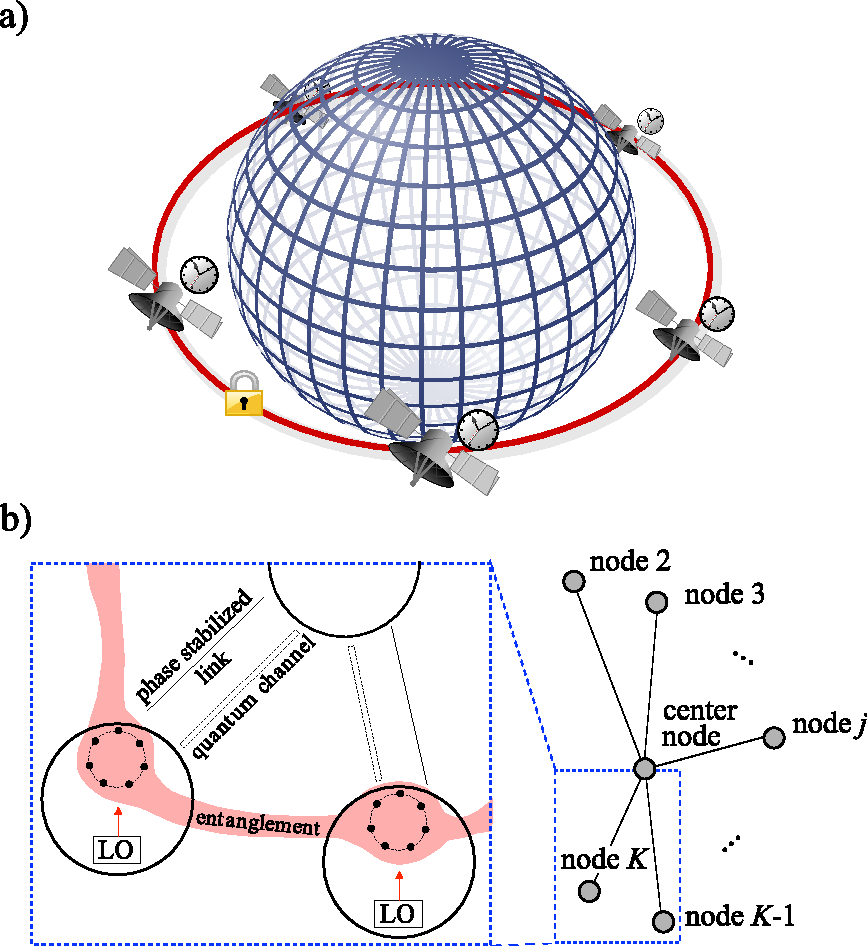
\includegraphics[width=0.8\textwidth]{./figs_Komar2014/fig1.pdf}
\caption
[The concept of world-wide quantum clock network]
{
\label{fig:1} The concept of world-wide quantum clock network.
a) Illustration of a cooperative clock operation protocol in which individual parties (e.g., satellite based atomic clocks from different countries) jointly allocate
their respective resources in a global network involving entangled quantum states. This guarantees an
optimal use of the global resources, achieving an ultra-precise clock signal
limited only by the fundamental bounds of quantum metrology and,
in addition, guaranteeing secure distribution of the clock signal.
 b) In addition to locally operating the individual clocks, the different nodes
 (i.e., satellites) employ network-wide entangled states to interrogate their
 respective local oscillators (LOs). The acquired information is sent to a particular node serving as
 a center where it is used to stabilize a center of mass mode of the different
 LOs. This yields an ultra-precise clock signal accessible to all network
 members.}
\end{figure}




% In the following, we describe the general working
% principle of  the proposed quantum clock network.



Each clock cycle consists of three stages: preparation of the clock atom state
(initialization), interrogation by the LOs (measurement) and correction of the
laser frequency according to the measurement outcome (feedback).
In the further analysis, we assume, for convenience, that in each interrogation
cycle one of the nodes plays the role of the center, which initiates
each Ramsey cycle and collects the measurement data from the other nodes via
classical channels [\reffig{fig:1}~b)], as well as LO signals via optical links,
 to feedback the COM signal.
(The role of the center can alternate to provide extra security, see
 Supplementary Information). This information, in turn, can be utilized in a feedback cycle to yield a Heisenberg-limited
stability of the COM clock signal generated by the network, which is 
subsequently distributed to the individual nodes in a secure fashion.  As a
result, after a few cycles, the LOs corresponding to each individual node
achieve an accuracy and stability effectively resulting from interrogating atoms
in the entire network.



\section{Preparation of network-wide entangled states}
\label{sec:NWES}

In the initialization stage of each clock cycle, entangled states spanning
across the nodes at different geographical positions of the network are
prepared. In the following, we describe exemplarily how a single network-wide
GHZ state can be prepared. 
The entangled states employed in the proposed quantum network protocol -- which
is described in the following section -- consist of products of GHZ states of
different size. They can be prepared by repetition of the protocol that
we now describe.

For simplicity, we assume that each node $j$ ($j=1,\dots K$) contains an
identical number $n$ of clock qubits which we label as $1_j, 2_j,\dots n_j$ (in
the Supplementary Information we discuss the case where the nodes contain
different amounts of clock qubits).
Further, we assume, for convenience, that the center node ($j=1$) has access to
additional $2(K-1)$ ancilla qubits $a_2,\dots, a_K,b_2,\dots,b_K$ besides the
$n$ clock atoms (a slightly more complicated procedure allows to refrain from
the use of ancilla qubits, see Supplementary Information).
The entangling procedure starts at the center with the creation of a fully
entangled state of one half of the ancilla qubits $\{b_j\}$, and its first clock
qubit $1_1$. 
This can be realized, e.g.  with a single qubit $\pi/2$-rotation
(on qubit $1_1$)
and a collective entangling operation, which is equivalent to a series of
CNOT gates \cite{Nielsen_Chuang} (between $1_1$ and each $b_j$).
The result is a GHZ state, $[\ket{00\dots 0}_{1_1,b_2,b_3,\dots b_K} +
i\ket{11\dots 1}_{1_1,b_2,b_3,\dots b_K}]/\sqrt{2}$.
%performed with the local oscillator field at the center, $\mathcal{E}_1$. 
% \bel
% 	\ket{00\dots 0}_{c_1,c_2\dots c_K} \quad\rightarrow\quad \frac{\ket{0}_1 +
% 	i\ket{1}_1}{\sqrt{2}} \ket{0\dots 0}_{2\dots M} \quad\rightarrow\quad
% 	\frac{\ket{00\dots 0}_{1,2\dots M} + i\ket{11\dots 1}_{1,2\dots M}}{\sqrt{2}},
% \eel
In parallel, the center uses the other half of the ancillas $\{a_j\}$ to create single EPR pairs with each node $j\neq1$,
either by directly sending flying qubits and converting them to stationary
qubits, or by using quantum repeater techniques to prepare high-fidelity entanglement \cite{duan3}. As a result of this procedure, 
one part of the pair is stored at the center node (qubit $a_j$), while the other one
is stored at the $j$th  node (qubit $1_j$), forming the states $[\ket{00}_{a_j,1_j} +
\ket{11}_{a_j,1_j}]/\sqrt{2}$ for every $j$ (see \reffig{fig:entangling}).
\begin{figure}
\centering
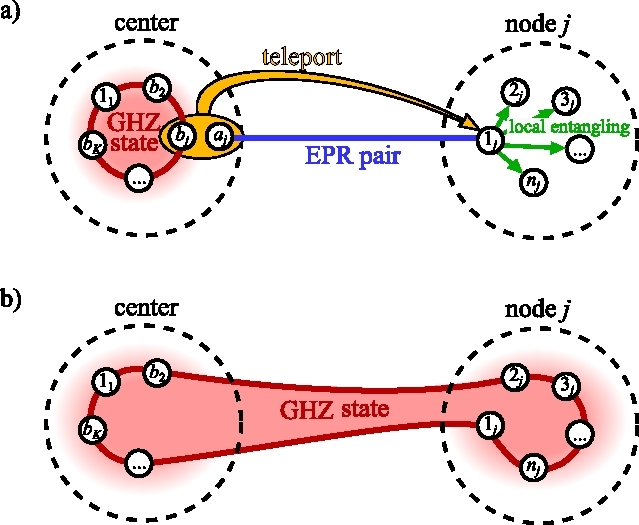
\includegraphics[width=0.7\textwidth]{./figs_Komar2014/fig2.pdf}
\caption
[Entangled state preparation between distant nodes]
{
\label{fig:entangling}
Entangled state preparation between distant nodes.
a) The center node $(j=1)$ initiates the initialization sequence by preparing a
local GHZ state across the qubits $\{b_j\}_{j=2}^K$ and $1_1$, as well as $(K-1)$ EPR pairs on
the qubit pairs $\{(a_j,1_j)\}_{j=2}^K$.
Quantum teleportation expands this GHZ state to the first qubit within each of
the individual nodes.
b) Originating from the teleported qubits, the nodes grow the GHZ state to
involve all the desired local qubits by employing local entangling
operations.
The procedure results in a common GHZ states over all atoms of the nodes.
 }
\end{figure}


%\subsection{Entangling}
% based on the existence of a secure central
% station,
Next, the center performs $K-1$ separate Bell measurements on
 its ancilla qubit pairs $\{(b_j, a_j)\}$. This teleports the state of qubit $b_j$ to
 qubit $1_j$
($j=2,\dots K$), up to a local single-qubit rotation, which is performed
after the measurement outcomes are sent to the node via classical channels.
The result of the  teleportations is a collective GHZ state
$\frac{1}{\sqrt{2}}\ket{00\dots 0}_{1_1,1_2,\dots 1_K} + i \ket{11\dots
1}_{1_1,1_2,\dots 1_K}$, stretching across the first qubits of all $K$ nodes.

In the final step of entangling, all nodes (including the center) extend the
entanglement to all of their remaining clock qubits. To do this, each node $j$
performs the collective entangling operation mentioned before based on
$1_j$ and targeting qubits $2_j, 3_j, \dots n_j$.  At the end of the protocol the different nodes share a common
GHZ state $[\ket{\mathbf{0}} + i\ket{\mathbf{1}}]/\sqrt{2}$, where
$\ket{\mathbf{0}}$ and $\ket{\mathbf{1}}$ are product states of all qubits
$\{i_j\;:\; i=1,2,\dots n,\; j=1,2,\dots K\}$ being in $\ket{0}$ or $\ket{1}$,
respectively. As discussed below, in practice the entanglement distribution can
be done  either via polarization- or frequency-entangled photons with frequency
difference in the microwave domain, in which case the ancillary qubits involved
in the entanglement distribution will be different from the clock qubits.
Typically, as part of the preparation process, time delays arise between the
initialization of different clock qubits. Its detrimental effects can be
entirely avoided by proper local timing or prior preparation of entanglement, as
discussed in the Supplementary Information.

\section{Interrogation}
\label{sec:SA}


The use of entangled resources 
% (in form of network-wide GHZ-like states) 
during
the interrogation phase enables an optimal use of the available resources via
the following procedure.  Assume we have a total of $\tilde N$ 
%($M$ being a positive integer)
qubits at
our disposal which are equally distributed between the $K$ nodes (indexed
$j=1,\hdots K$) and prepared in a non-local GHZ state $[\ket{\mathbf{0}} +
i\ket{\mathbf{1}}]/\sqrt{2}$, where $\ket{\mathbf{0 (1)}}\equiv\ket{0(1)}^{\otimes
\tilde N}$. During the
interrogation time $T$, a clock qubit at node $j$ picks up a relative phase $\phi_j = \delta_j
T$.
Due to the non-local character of the state, these phases accumulate in the total
state of the atoms  $[\ket{\mathbf{0}} + i e^{i\Phi}\ket{\mathbf{1}}]/\sqrt{2}$,
where the collective phase after the interrogation time $T$ is given as
\bel
\label{eq:1}
\Phi = \sum_{j=1}^K \frac{\tilde N}{K} \phi_j =
\tilde N \delta_\mathrm{COM} T,
\eel
where $\delta_\mathrm{COM} = \nu_\mathrm{COM} - \omega_0$.
% \bel
% 	\frac{1}{\sqrt{2}} \big(\ket{\mathbf{0}} + i
% 	e^{i\Phi}\ket{\mathbf{1}}),\qquad \Phi = \sum_{k=1}^M N_k \delta_k T .
% \eel
% This phase, $\Phi$, is sensitive to the weighted average of the detunings, ie.
% the center of mass of the detunings, $\nu_\mathrm{COM}-\omega_0 =
% \delta_\mathrm{COM} = [\sum N_k \delta_k] / [\sum N_k]$. By designing a
% measurement scheme estimating $\Phi$, we can get information on this COM
% detuning.
To extract the phase information picked up by the different GHZ states, 
% after each interrogation phase, 
the individual nodes $j$ measure their respective
qubits in the $x$-basis, and evaluate the parity of all measurement outcomes
$p_j$.
Subsequently, the nodes send this information to the center node via a classical
channel, where the total parity $p = \prod_{j} p_{j}$ is evaluated, and the
phase information is extracted \cite{Bollinger1996, Leibfried2004}. Note, that
only the full set $\{p_j |j=1\hdots K \}$ contains information. 
% This can be
% interpreted as only the center node holding the key,  namely its own measurement
% outcome $p_1$, to decode the phase information sent from the nodes.

The proportionality with $\tilde N$ in \refeq{eq:1} represents the quantum
enhancement in the estimation of $\delta_\mathrm{COM}$. However, for realistic
laser noise spectra, this suggested enhancement is corrupted  by the increase of
uncontrolled phase slips for a single GHZ
state 
%(i.e., undetectable transitions between fringes in a Ramsey
%experiment) 
\cite{Wineland1998}: Whenever, after the Ramsey time $T$, the phase $\Phi$ --
which due to the laser frequency fluctuations constitutes a random variable itself --
falls out of the interval $[-\pi,\pi]$ the estimation fails. This limitation
restricts the maximal Ramsey time to values $T < (\tilde
N\gamma_\mathrm{LO})^{-1}$, preventing any quantum gain in the estimation.


To circumvent this problem, we use entangled states consisting of products of
successively larger GHZ ensembles, see SI and 
\cite{Kessler2014}. In this approach, 
% interrogated network 
atoms are split into
several independent, shared groups.
% enables to correct for laser phase slips and 
%restores the quantum
%enhancement [REF:PRL paper]. 
% In the following, we apply these ideas to the clock network
% described above.
We write the number of the first group of atoms as $\tilde N =2^{M-1} K$, for
some natural number $M$.
Furthermore, the network shares additional groups of atoms, each containing
$2^{j} K$ ($j=0, \hdots M-2$) equally distributed between the nodes and prepared
in GHZ states. 
% \pk{The state of all the qubits can be written as
% $\left(\prod_{j=0}^{M-1} [\ket{0}^{2^jK} +
% i\ket{1}^{2^jK}]/\sqrt{2}\right)^{n_0}$, where $n_0$ is a small integer.}
Additionally, each node has a small number of uncorrelated atoms interrogated by
the LOs. Using a protocol reminiscent of the phase estimation algorithm
\cite{Kessler2014,Nielsen_Chuang, Giedke2006}, measurement results from each
level $j$ allow to directly assess the bits $Z_j \in \{0,1\}$ of the binary
fraction representation of the laser phase $\Phi_\mathrm{LO}=\delta_\mathrm{COM} T
=2\pi [(Z_1-1) 2^{-1} + Z_2 2^{-2} + Z_3 2^{-3} \hdots]$.
(See SI, section I.B for details.)
This
% accounts for all phase slips {\it what does this mean?? up to the uncorrelated
% ensemble}, and
yields an estimate of $\Phi_\mathrm{LO}$ with Heisenberg-limited accuracy, up to a
logarithmic correction, see SI:
\bel 
	\Delta \Phi_\mathrm{LO} =\frac{8}{\pi}\log(N)/N,
	\label{eq2}
\eel 
even for Ramsey times beyond the limits of the laser frequency fluctuations [$T
> (\tilde N\gamma_\mathrm{LO}^{-1})$], where $N$ represent the total number of
clock atoms employed in the scheme. The logarithmic correction arises due to the
number of particles required to realize this (incoherent) version of the phase
estimation algorithm.

\section{Feedback}

The measured value of the phase  $\Phi_\mathrm{LO}$,
gives an estimate on the COM detuning
$\tilde\delta_\mathrm{COM}$ after each Ramsey cycle, which is subsequently used
by the center node to stabilize the COM laser signal.
To this end, the center generates the COM of the frequencies. Every node sends
its local oscillator field $\mathcal{E}_i$ to the center via phase-stable
optical links, and the center synthesizes the COM frequency $\nu_\mathrm{COM}$ by
averaging the $\nu_j$ frequencies with equal weights.
% \footnote{With different
% number of qubits at each node, the weighted average needs to be taken.}
This can be implemented via heterodyne beat of the local oscillator in the
center against each incoming laser signal, resulting in $K$ beat frequencies.
Synthesizing  these beat frequencies allows the
local oscillator of the central node to phase track $\nu_\mathrm{COM}$.
%Subsequently, the center uses the 
%acquired information about $\delta_\mathrm{COM}$ to stabilize $\nu_\mathrm{COM}$ by
%application of digital frequency shifts. 
The center distributes the stabilized clock signal to different members of the network by sending individual error
signals $\tilde \delta_j = \tilde \delta_\mathrm{COM} + (\nu_j - \nu_\mathrm{COM})$
to all nodes $j$, respectively, and corrects its own LO as well, accordingly.
Alternatively, the center can be operated to provide restricted feedback
information to the nodes, see SI.



\section{Stability analysis}
\label{sec:comp}

In this section, we demonstrate that the proposed quantum clock network achieves
the best clock signal, allowed by quantum theory for the available resources, i.e.
the total atom number. 
% Rather than individually operating their respective LOs the
% joint use of resources allows the network to  directly interrogate and stabilize
% the COM mode of the lasers. 
To quantify this cooperative gain, we compare
networks of different types (classical or quantum mechanical interrogation of
the respective LOs) and degrees of cooperation (no cooperation, classical, or
quantum cooperation).


First, we analyze the stability of the proposed quantum clock network,
corresponding to the case of quantum interrogation and cooperation (curve a in
\reffig{fig:comp}). In this case, the analysis resulting in \refeq{eq2}
suggests that near Heisenberg-limited  scaling with a total atom number can be achieved
for the entangled clock network. 
In particular, for a given total particle number $N$ and for averaging times
shorter than the timescale set by individual qubit noise $\tau < 1/(\gamma_i N)$
(where $\gamma_i$ is the atomic linewidth, the factor $N$ results from the
enhanced decoherence of the entangled interrogation state
\cite{Huelga1997}), the network operation achieves a Heisenberg-limited Allan
deviation (ADEV) of the COM laser mode
\begin{align}
\label{eq:ADEV1}
 	\sigma_y(\tau) 
%  	=  \frac{1}{\omega_0 \sqrt{n_0}2^{M}K} \frac{1}{\tau}
	\sim \frac{ \sqrt{\textrm{log}(N)}}{\omega_0 N} \frac{1}{\tau},
\end{align}
up to small numerical corrections [cf. SI].
% Here, the number of GHZ copies per group $n_0\sim \textrm{log}(N)$ ($N\approx n_0
% 2^{M+1} K $) is found after optimization, and
% gives rise to a logarithmic correction in the total particle number.
The $1/\tau$ scaling results from the effective cancellation of the low
frequency part of the laser noise spectrum, achieved
by the cascaded protocol described above, possibly in combination with additional stages of uncorrelated interrogations using varying Ramsey times \cite{Rosenband2013,Borregaard2013}, see \cite{Kessler2014}.
This allows the cycle time $T$ (which is assumed to be equal to
the interrogation time) to be extended to the total available measurement time
$\tau$.
\begin{figure}
\centering
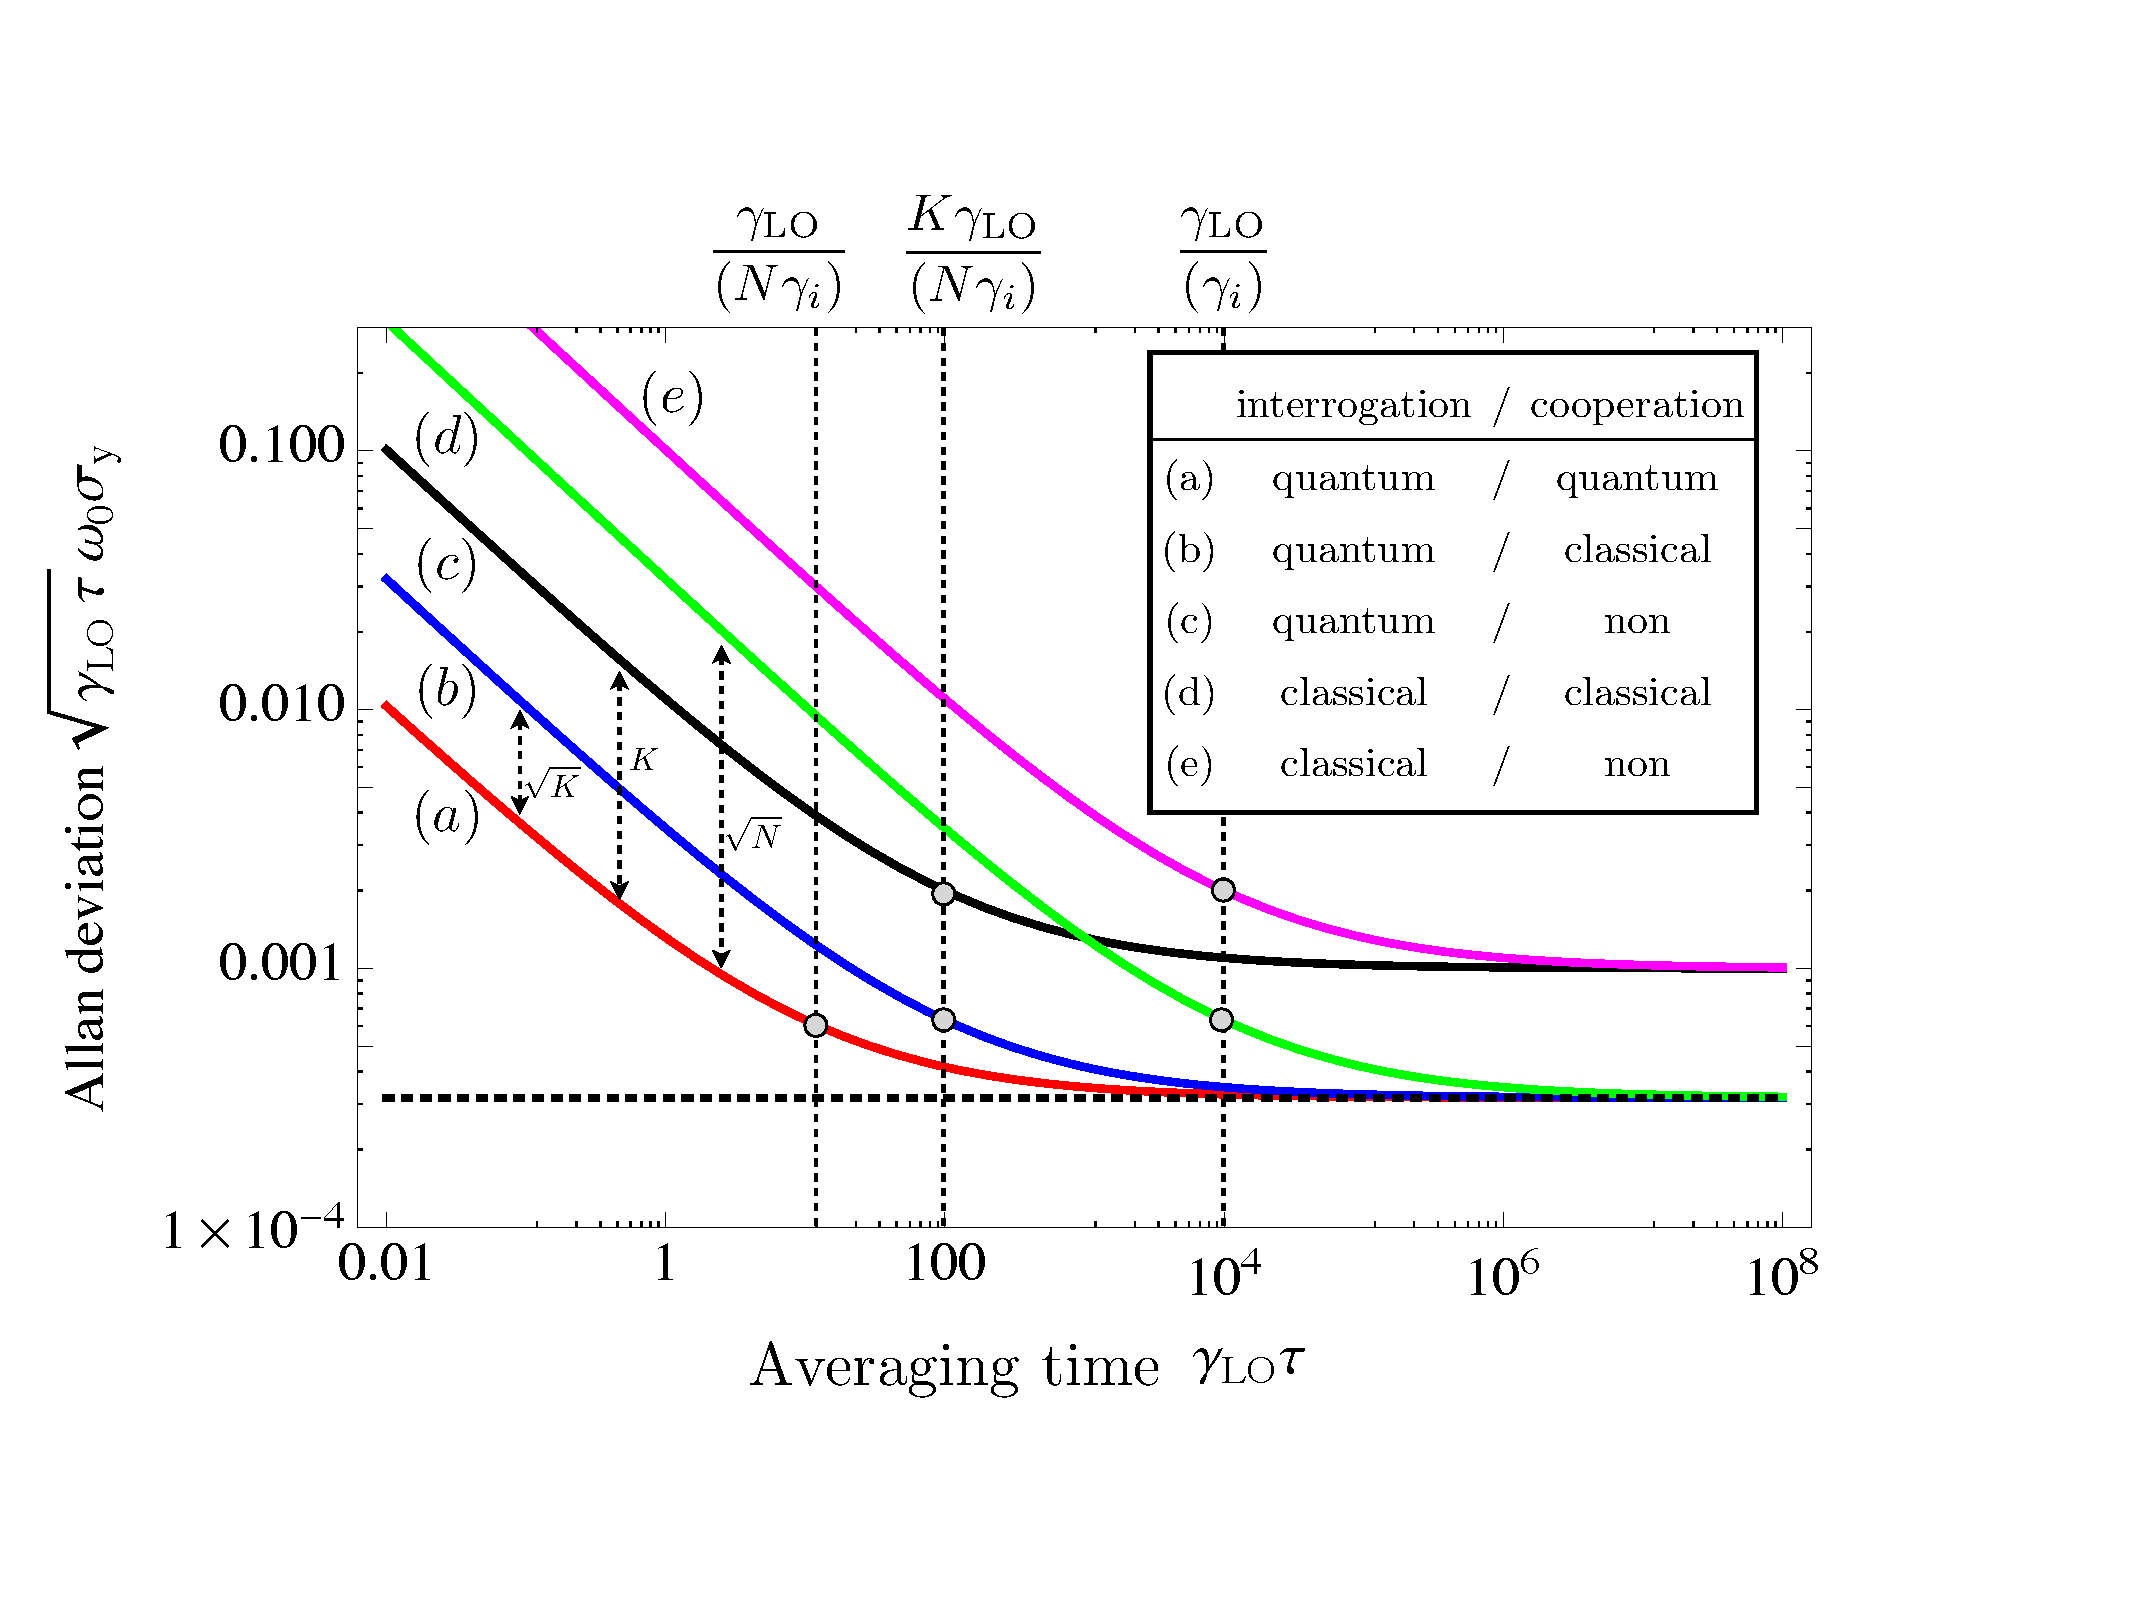
\includegraphics[width=1\textwidth]{./figs_Komar2014/fig3.pdf}
\caption
[Performance of different operation schemes]
{
\label{fig:comp}
Performance of different operation schemes. Comparison of
the achievable (rescaled) Allan deviation $\sqrt{\gamma_\mathrm{LO} \tau} \omega_0 \sigma_y$ using clock networks of different types and degrees of
cooperation. (a) the proposed protocol realizing quantum interrogation and
cooperation, (b) quantum interrogation and classical cooperation, (c) quantum
interrogation and no cooperation, (d) classical interrogation and classical
cooperation, (e) classical interrogation and no cooperation (cf. text). The
dotted base line represents the fundamental bound arising from the finite width
of the clock atoms transition
[compare \refeq{eq:ADEV2}]. This optimal stability can be attained only via cooperation between the
nodes.
The quantum clock network (a) represents the optimal form of cooperation, and reaches this boundary faster than any other
operational mode. Parameters are $N=1000$, $K=10$, $\gamma_i=10^{-4}\gamma_{LO}$.
 }
\end{figure}



Eventually, for large averaging times $\tau > 1/(\gamma_i N)$ the
Ramsey time becomes fundamentally limited by individual
noise processes that determine the atomic linewidth $T\leq 1/(\gamma_i N)$.
As a result, the $1/N$ scaling breaks down, and the ADEV returns to the square
root scaling with both the employed particle number and averaging time,
\begin{align}
\label{eq:ADEV2}
	\sigma_y(\tau) \sim \frac{ 1}{\omega_0 \sqrt N}
	\sqrt{\frac{\gamma_i}{\tau}},
\end{align}
up to constant numerical factors.  \refeq{eq:ADEV2} results from fundamental
quantum metrological bounds \cite{Escher:2011fn} (In the case of
dominating trap losses, the loss rate simply replaces $\gamma_i$ in the above
formula.), and represents the best conceivable clock stability in the presence
of individual particle decoherence which, in a network, can only be achieved via cooperation. Independently operating a clock, in contrast, can only achieve a stability scaling with the local number of atoms, i.e. $\sigma_y(\tau)\propto \sqrt{K/N}$.


 \reffig{fig:comp} illustrates the comparison of entangled clock network with
other approaches.
A network in which the $K$ nodes cooperate classically (curve b in
Fig.~\ref{fig:comp}), by locally measuring the individual phase deviation
$\phi_j$, and combining the outcomes via classical channels, outperforms
individually operated clocks (curve c) by a factor of $\sqrt K$ 
(for both cases, assuming optimal
quantum interrogation for individual nodes
\cite{Kessler2014,Borregaard2013_nearHeisenberg}).
The quantum network protocol (curve a)
increases this cooperative advantage by an additional factor of $\sqrt K$ for
short averaging times, reaching Heisenberg-limit, Furthermore the ADEV
converges to the fundamental bound [\refeq{eq:ADEV2}] $K$ times faster compared
to the case of classical cooperation (curve b).
Although an optimal, classical, local protocol
(e.g. \cite{Rosenband2013, Borregaard2013}), combined with classical
cooperation (curve d), eventually reaches the same
bound [\refeq{eq:ADEV2}],
% in this case, the obtainable stability is always
 % limited by the standard quantum limit with regard to the
% employed resources, $\sigma_y(\tau) \propto 1/\sqrt N$. Therefore,
this approach is atom-shot noise limited, and hence its stability is reduced by
a factor of  $\sqrt N$ for short averaging times [compare \refeq{eq:ADEV1}]
compared to the quantum network protocol.  Hence, the optimal stability
[\refeq{eq:ADEV2}] is reached at averaging times that are $N$ times longer
than for the proposed quantum network. Naturally, all of the above approaches
are superior to a classical scheme without cooperation (curve e).

As a specific example, we first consider ion clocks that can currently achieve a
stability of $2.8\times 10^{-15}$ after $1~\mathrm{s}$ of averaging time
\cite{Chou2010}. The entangled states of up to 14 ions has already been
demonstrated \cite{Monz2011} as was the entanglement of remote ions
\cite{Maunz2007}. We consider a network of ten clocks, each containing ten ions.
Using $\mathrm{Al}^+$ ($\omega_0 = 2\pi \times 1121~\mathrm{THz}$, $\gamma_i = 2\pi
\times 8~\mathrm{mHz}$), we find that the quantum cooperative protocol can reach
$4\times 10^{-17}$ fractional frequency uncertainty after $1~\mathrm{s}$. Larger
improvements could potentially be achieved using e.g. $\mathrm{Yb}^+$ ions, due to the long coherence time ($2.2\times
10^4~\mathrm{s}$) of its octupole clock transition.

The quantum gain could be even more pronounced for neutral atomic clocks. For a
network consisting of ten clocks similar to the one operated in JILA
\cite{Bloom2013}, each containing 1000 neutral atoms with central frequency
$\omega_0 = 2\pi\times 429~\mathrm{THz}$ and linewidth $\gamma_i = 2\pi \times
1~\mathrm{mHz}$,  the quantum cooperative scheme can achieve a stability of $\sim
2\times 10^{-18}$ after 1s averaging, and is an order of magnitude
better than the best classical cooperative scheme.  Future advances,
employing clock transitions with linewidths of a few tens of
$\mu\mathrm{Hz}$ (such as erbium), could possibly allow for further
improvement, achieving fractional frequency uncertainty beyond $10^{-20}$
after $\tau \sim 100~\mathrm{s}$. This level of stability is in the same order of
magnitude as the required sensitivity to successfully use the network as a
gravitational interferometer \cite{Schiller2008}.


So far we have assumed perfect operation and infinitely fast entanglement
distribution rates. In the SI we analyze these assumption and find that the
advantage of our scheme persists provided that fidelity  of the local collective
entangling \cite{MSgate} (which creates a GHZ state of $N/K$ qubits) exceeds the
threshold fidelity $F_\mathrm{th}$, where $1-F_\mathrm{th} \sim 1/(K\log N)$, and
the EPR sharing rate is higher than $R_\mathrm{EPR}\sim (\log N)^2 \gamma_i$.
For the optical clock example presented above, $F_\mathrm{th} \sim 0.99$, and
$R_\mathrm{EPR} \sim 1~\mathrm{Hz}$. While local operations with fidelity
$\sim 0.95$ have been realized for $N\sim 5$ ions \cite{Monz2011}, the errors
in such operations increase with $N$, making this realization more challenging.




\section{Security}
\label{sec:Security}
A network with such precise time-keeping capabilities can be subject to both internal
and external attacks. Effectively countering them is crucial to establish a
reliable ground for cooperation. We consider the network secure if the
implemented countermeasures can prevent external parties from benefiting from
the network (eavesdropping), as well as effectively detect any malicious activities of any of the members (sabotage).

Sabotage describes the situation where one of the nodes -- intended or
unintended -- operates in a damaging manner. For example, one node
% that is blatant enough to not comply with the formal requirements of the
% protocol is easily detected by the center within the time period of a single
% cycle, and then the particular node gets excluded from further cycles. More
% stealthy types of sabotage
could try sending false LO frequencies or wrong measurement bits in the hope of
corrupting the collective measurement outcomes. In order to detect such
malicious participants, the central node can occasionally perform assessment
tests of the different nodes by teleporting an uncorrelated qubit state
$[\ket{0} + e^{i\chi}\ket{1}]/\sqrt{2}$, where $\chi$ is a
 randomly chosen phase known only to the center. By checking for statistical
discrepancies between the measurement results and the detuning of the LO signal
sent by the node under scrutiny, the center can rapidly and reliably determine
whether the particular node is operating properly (See \reffig{fig:security}a
and Supplementary Information),
however this strategy breaks down, if multiple sabotage attacks
happen within a short time.
\begin{figure}
\centering
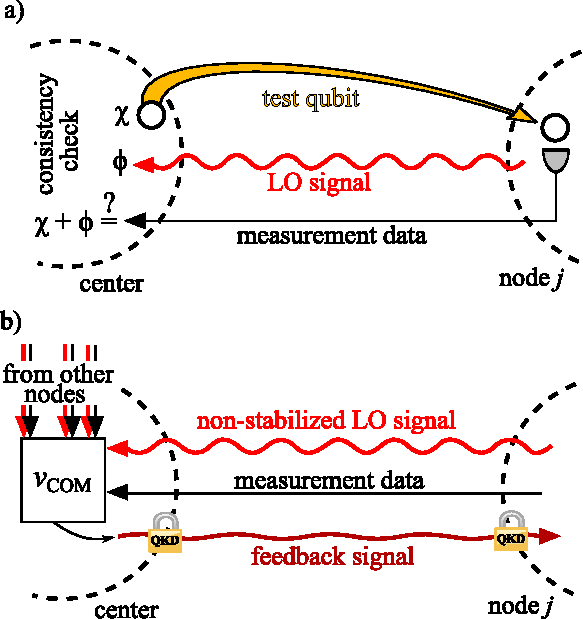
\includegraphics[width=0.7\textwidth]{./figs_Komar2014/fig4.pdf}
\caption
[Schematics of security countermeasures]
{
\label{fig:security}
Schematics of security countermeasures.
a) The center node can choose to test any node $j$ by teleporting a disentangled
qubit with a certain phase rotation. A properly operating node creates a local
GHZ state $[\ket{\mathbf{0}} + e^{i\chi}\ket{\mathbf{1}}]/\sqrt{2}$ from the
sent qubit,
 measures the parity of the GHZ state, and sends it to the center. The
measured parity holds information on the phase $\phi' = \chi + \phi$, where
$\phi$ is the accumulated phase of the LO at the node. The center verifies
$\phi$ by comparing it with the classically determined  phase of the sent LO
signal with respect to the COM signal.
b) Eavesdropping can be prevented by prescribing that only the non-stabilized LO
signals are sent through  classical channels and encoding the radio frequency
feedback signal with phase  modulation according to a shared secret key.
}
\end{figure}


Eavesdropping, i.e., the unauthorized attempt to access the stabilized
$\nu_\mathrm{COM}$ frequency, can be prevented by encoding the classical channels,
over which the center and the nodes exchange feedback signals, using quantum key
distribution protocols \cite{Gisin2002}. Our protocol can keep the stabilized
signal hidden from outsiders by mixing the feedback signal with the LO signal at each node only
after the non-stabilized LO has been sent to the center (see
\reffig{fig:security}b and SI). As a result, even if  all LO signals are intercepted, the eavesdropper is able to access
only the non-stabilized COM signal. Furthermore, the center exclusively can decode the
measurement results sent by the individual nodes using its own measurement outcomes as mentioned above. 
As a result, the stabilized COM signal remains
accessible exclusively to parties involved in the collaboration.

Finally, we note that a distributed operation offers significant security
advantages over an alternative approach of having all resources combined in one
place from where the signal is distributed. In case of a physical attack of the
network, disabling the center or the communication links, the nodes can fall
back to an independent clock operation using their local resources.

\section{Outlook}

One of the advantages of the proposed quantum clock network involves its ability
to maintain and synchronize the time standards across multiple parties in
real-time. 
% This can be achieved with classical cooperation schemes as well,
% however it arises naturally in the quantum scheme. 
Unlike the current world time standard, where the individual signals from
different clocks are averaged and communicated with a time delay (a so called
paper clock), in our quantum clock network all participants have access to the
ultra-stable signal at any time.
This makes it possible to measure systematic errors of different clocks in
real time, which in turn allows to correct them \cite{Bloom2013}, unlike in the
case of the paper clock which has to rely on the retrospectively averaged time 
signals (see SI). 
The enhanced stability of the network signal hereby allows for longer Ramsey
times in the control measurements used to determine the systematics of the
single clock.
% The longer Ramsey time allows this measurement to be carried
% out with precision limited only by the accuracy of the network.
Furthermore, by having full access to their local clocks the different parties
keep  their full sovereignty and ensure security, as opposed to a joint
operation of a single clock.

Realization of the full-scale network of the type described here will require a
number of technological advances in both metrology and experimental quantum
information science. 
% Practical realization can be based on optical atomic 
% clocks involving either trapped ions \cite{Chou2010} or neutral atoms
% \cite{Nicholson2012}.
% While ions provide a more straightforward implementation of the preparation of entangled qubit states \cite{Cirac2000, Monz2011}, state of the art neutral atom clocks
% feature large atom number resulting in better stability and potentially more
% significant quantum enhancement \cite{Nicholson2012}.
The remote entanglement can be implemented by using recently demonstrated
techniques for individual atom-photon entanglement \cite{Olmschenk2009,
Chou2007, togan, Bernien2013, Riste2013}. Since the teleportation protocol
requires quantum links capable of sharing EPR pairs with sufficiently high
repetition rate and fidelity, entanglement purification \cite{Dur1999} and
quantum repeater techniques \cite{duan3} will likely be required. In
practice, qubits used for entanglement distribution may not be ideal for clocks.
 However, as noted previously  remote entanglement does not need to involve
coherent qubits at optical frequencies (e.g., polarization entanglement can be
used). In such a case,   the use of hybrid approaches, combining  different
systems for entanglement and local clock operations, may be warranted.
Similarly, signals from clocks employing different transition frequencies
can be coherently connected by frequency combs, allowing clocks with different
clock qubits to participate.
% So far we have considered schemes requiring individual qubit addressing, however
It might also be interesting to explore if high-fidelity entangled EPR pairs can
be used to create remote entangled states of spin-squeezed type \cite{Leroux2010,
Sherson2006, Ma2012}, or by following the proposed approach for cat state
preparation in atomic ensembles \cite{McConnell2013}, 
or using collective interactions (such as \cite{MSgate}) and repetitive teleportation 
\cite{Andersen2013}.
% Alternatively, recently demonstrated  individual addressing in optical lattices
% \cite{Bakr2009, Lee2013} could be combined with entanglement swapping techniques
% to directly entangle optical lattice clocks.
% Lastly, the use of a continuous variable approach can be potentially explored to
% create squeezed atomic states across the network \cite{Sherson2006, Ma2012}. The
% use of collective measurements may allow one to reach Heisenberg limited
% stability \cite{Borregaard2013_nearHeisenberg}, while  squeezing can be transferred
% from photons to atomic ensembles \cite{Sherson2006, Hammerer2010}. An important
% open question of sensitivity of these techniques to photon losses needs to be
% addressed. 
In addition, while space-based communication networks will be capable
of maintaining optical phase coherence for the links between clocks, we note
that establishing ground-space coherent optical links remains a technical
challenge and requires an intense research effort which has recently started
\cite{Djerroud2010}.
% Beyond specific implementations, a number of other research directions may be
% explored. These include optimal eavesdropping, error correction and security
% strategies, robust feedback approaches minimizing technical imperfections such
% as Dick effect \cite{Santarelli1998}, as well as novel applications taking
% advantage of enhanced clocks with short averaging time.
Finally, if the entire network is spanned by satellites in space, the on-board
local oscillators can further benefit from the much lower noise level compared
to ground-based clocks.

If realized, such a quantum network of clocks can have important scientific,
technological, and social consequences. Besides creating a world platform for
time and frequency metrology, such a network may find important applications to
a range of technological advances for earth science \cite{Tapley2005},
precise navigation of autonomous vehicles and space probes (requiring high
 refresh rate), and to the test and search for the fundamental laws of
nature, including relativity and the connection between quantum and
gravitational physics \cite{Abramovici1992, Seidel2007, Schiller2008, Wolf2008}.
In order to explore these exciting applications one can either use the excellent
common frequency reference generated by the clock network, or, alternatively,
prepare modified collective states of different nodes that can directly measure
the specific signal under study. 
 







  
% Chapter 8:
\chapter{Entangling collective Rydberg excitations of remote atomic ensembles}
\label{ch:Komar2015}
%%%%%%%%%%%%%%%%%%%%%%%%%%%%%%%%%%%%%%%%%%%%%%%%

\section{Introduction}
From \cite{}


\appendix
\dsp 
\chapter{Appendices for Chapter \ref{ch:Komar2013}}
\label{app:Komar2013}

\section{Derivation of reflected mode operator}
\label{App: Reflection}

We obtain the reflected mode operator $c_R$ using input-output
relations for a two-sided cavity. 
By assuming that the two endmirrors have
the same transmittivity ($\propto\kappa$), we can write the input-output
relation for cavity mode $c_a$ on the driven mirror as
\bel
	c_{a,\text{out}} =
	\sqrt{\kappa}c_a - c_{a,\text{in}},
\eel
where $c_{a,\text{in}} = -i\frac{\Omega}{\sqrt{\kappa}}$ is the incoming field
operator on the mirror and $c_{a,\text{out}}$ is the output field operator.
For direct comparision with $c_a$ we
divide by $\sqrt{\kappa}$ and define the
reflection mode operator as  
$c_R \equiv c_{a,\text{out}}/\sqrt{\kappa} =
c_a +i\frac{\Omega}{\kappa}$.


\section{Analytic model}
\label{sect:App:steady_state}


%\label{sec:analytic_model}


In this appendix we provide the analytic solutions
used to calculate one- and two-time
correlation functions in steady state.
First, one-time correlations are calculated
from  the steady state solutions of
Eqs.~(\ref{eq:c000}--\ref{eq:c022}).
We set the time derivatives to zero and
solve the equations iteratively,
order by order in the weak drive.
This procedure yields
\bal
	\label{eq:alpha000}\bar A_{000} &\approx& 1,\\
	\label{eq:alpha100}\bar A_{100} &=& -i\alpha \frac{1}{1 + 4x^2},\\
	\label{eq:alpha011}\bar A_{011} &=& -\alpha \frac{2x}{1 + 4x^2},\\
	\label{eq:alpha200}\bar A_{200} &=& -\frac{\alpha^2}{\sqrt{2}}\frac{1 + 2x^2}{(1 +
	4x^2)(1 + 6x^2)},\\
	\label{eq:alpha111}\bar A_{111} &=& i\alpha^2\frac{2x}{(1 + 4x^2)(1 + 6x^2)},\\
	\label{eq:alpha022}\bar A_{022} &=& \alpha^2\frac{4x^2}{(1 + 4x^2)(1 + 6x^2)},
\eal
where $\alpha = \Omega/\tilde\kappa$ ($|\alpha|^2 \ll 1$), $x = g/(4\tilde\kappa)$ and
$\tilde \kappa = \kappa -i\Delta$.  
Using these amplitudes, we can express all
equal time averages.
The mean photon numbers are
\bal
	\bar n_a &=& |\bar A_{100}|^2 ,\\
	\bar n_s &=& |\bar A_{011}|^2 ,\\
	\bar n_R &=& \left|\bar A_{100} + i\frac{\Omega}{\kappa}\right|^2,
\eal 
and the photon-photon correlation functions are
\bal
\label{eq:g2aa0}
	g^{(2)}_{aa}(0) &=& \frac{2|\bar A_{200}|^2}{|\bar A_{100}|^4},\\
\label{eq:g2ss0}
	g^{(2)}_{ss}(0) &= & \frac{2|\bar A_{022}|^2}{|\bar A_{011}|^4},\\
\label{eq:g2AA0}
	g^{(2)}_{RR}(0) &= &
	\frac{\left|-\left(\frac{\Omega}{\kappa}\right)^2+
	2i\frac{\Omega}{\kappa}\bar A_{100} +
	\sqrt{2}\bar A_{200}\right|^2}
	{\left|i\frac{\Omega}{\kappa}+\bar A_{100}\right|^4}.
\eal
To
leading order in $\kappa/g$ these
yield Eqs.~(\ref{eq:na}--\ref{eq:g2AA}).


At finite temperature we calculate steady state amplitudes
within each phonon subspace $n$ similarly
in the ansatz of \refeq{eq:psi_thermal}.
Using the  notation $R_\kappa(\omega)$ introduced 
in Section \ref{sec:onetime_correlation},
the steady state amplitudes
within the subspace with $n$ phonons in the optical
groundstate are
\begin{align}
%p_{1,0,n}=
|\bar A_{10n}|^2=&\frac{\Omega^2\sqrt{R_\kappa(0)}}
{R_{\kappa}\left(\frac{g}{2}\sqrt{n+1}\right)},\\
|\bar A_{01n+1}|^2=&\frac{\Omega^2 g^2 (n+1) }{4
R_{\kappa}\left(\frac{g}{2}\sqrt{n+1}\right)},\\
|\bar A_{20n}|^2 =&\frac{ \Omega^4
R_\kappa(g/\sqrt{8})}{R_\kappa\left(g\sqrt{(2n+1)/8}\right)R_\kappa\left(\frac{g}{2}
\sqrt{n+1}\right)},\\
|\bar A_{02n+2}|^2 =&\frac{ \Omega^4 g^4 (n+1) (n+2)}{32
R_\kappa\left(g\sqrt{(2n+1)/8}\right)R_\kappa\left(\frac{g}{2}
\sqrt{n+1}\right)}.
\end{align}


Two-time correlation functions are calculated similarly,
using the conditional state after a jump
(see Eqs.~(\ref{eq:psi^a}) and (\ref{eq:psi^s}))
as the initial condition.
For example the
unnormalized state after detection of a photon in the
$c_a$ mode is $c_a\ket{\psi} =  \bar A_{100}\ket{000} +
	\sqrt{2}\bar A_{200}\ket{100} + \bar A_{111}\ket{011}$. 
We solve
Eqs.~(\ref{eq:c000}--\ref{eq:c011}) for the amplitudes 
with this state as initial
condition.
The finite delay correlation of the driven mode is
\bel
\begin{split}
	&g^{(2)}_{aa}(\tau) = \frac{|A_{100}(\tau)|^2}{|\bar A_{100}|^4}.
\end{split}
\eel
in good agreement with the numerics.
The correlation of the undriven
mode $g^{(2)}_{ss}(\tau)$ is calculated similarly. 
The unnormalized
state after detection in the $c_s$ mode is  $c_s\ket{\psi} = 
\bar A_{011}\ket{001}  + \bar A_{111}\ket{101} +  \sqrt{2}
\bar A_{022}\ket{012}$.
Using this  as the
initial
condition we solve Eqs.~(\ref{eq:c001}--\ref{eq:c012}) for the amplitudes
in the conditional state. 
In the limit of $\gamma \ll \kappa$ we obtain
\bel
	g^{(2)}_{ss}(\tau) 
	=
	\frac{|A_{012}(\tau)|^2}{|\bar A_{011}|^4}.
\eel 


\chapter{Appendices for Chapter \ref{ch:Stannigel2012}}
\label{app:Stannigel2012}


\section{Phonon nonlinearities}

In Eq. (8) in the main text we have derived an effective master equation (ME) to
describe the nonlinear interaction between two phonon modes. In the following we
present an alternative, more rigorous, approach, which illustrates the
individual approximations made in the derivation of the effective phonon
nonlinearity in more detail. We first consider only a single mechanical mode,
e.g. $b\equiv b_1$, which also allows us more easily to compare the results with
exact numerical calculations of the full model.


\subsection{Model}

We start with the full ME for the two optical modes coupled to a single
resonator mode, which in the frame of the driving frequency $\omega_L$ can be
written as
\begin{equation}\label{eq:SM_ME}
\dot \rho = -i[H_0+H_g+ H_\Omega(t),\rho] + \mathcal{L}_{\rm diss} \rho. \\
\end{equation}
Here 
\begin{equation}
H_0=  \omega_m b^\dag b - \Delta_s c_s^\dag c_s - \Delta_a  c_a^\dag c_a, 
\end{equation}
and
\begin{equation}
H_g= \frac{g_0}{2} \left(c_a c_s^\dag b^\dag +    c_a^\dag c_s  b \right),
\end{equation}
are the free evolution and the OM coupling, respectively,  $H_\Omega(t)=
i\Omega_s(t) (c_s^\dag - c_s)$ is the driving field for the symmetric mode with
slowly varying amplitude $\Omega_s(t)$ and
\begin{equation}
\mathcal{L}_{\rm diss} \rho  = \sum_{\eta=s,a} \kappa \mathcal{D}[c_\eta] \rho +
\frac{\gamma}{2} \mathcal{D}_{\rm th}[b]  \rho,
\end{equation}
accounts for dissipation. Here we have defined the superoperator
$\mathcal{D}_{\rm th}[b] = (N_{\rm th}+1)  \mathcal{D}[b] +  N_{\rm th} 
\mathcal{D}[b^\dag]$ to describe the coupling to a thermal bath.



\subsection{Displaced frame}

In contrast to the approach outlined in the main text, we now start our analysis
with a unitary displacement $U(t) c_sU^\dag (t)= c_s +\alpha(t)$ where the
classical cavity field $\alpha(t)$ obeys
\begin{equation}
\dot \alpha(t)= (i\Delta_s - \kappa) \alpha(t)  + \Omega_s(t). 
\end{equation}�
This unitary transformation eliminates the classical driving field and in the
new frame the resulting ME can be written as
\begin{equation}\label{eq:SM_FullME}
\begin{split}
\dot \rho = &-i[H_{\rm lin}+H_g,\rho] + \mathcal{L}_{\rm diss} \rho, \\
\end{split} 
\end{equation}
where $H_\Omega(t)$ has disappeared, but the linear part of the Hamiltonian now
contains an additional coupling between the resonator and the anti-symmetric
cavity mode,
\begin{equation}\label{eq:Hlin}
H_{\rm lin}�=  H_0  + G(t) c_a b^\dag + G^*(t) c_a^\dag b,
\end{equation} 
where $G(t)=g_0 \alpha(t)/2$. Note that ME \eqref{eq:SM_FullME} is still exact
and we will use this equation for our exact numerics below.


\subsection{Hybridized modes}

To proceed, we assume that $\alpha(t)$ is constant or slowly varying on the
timescale set by the detunings $|\Delta_a+\omega_m^i|$. This allows us to write
$H_{\rm lin}$ in its adiabatic eigenbasis
\begin{equation}
H_{\rm lin}�= - \Delta_s c_s^\dag c_s  - \tilde \Delta_a C^\dag C + \tilde
\omega_m B^\dag B,
\end{equation}
where  the $C$ and $B$ are bosonic operators for the hybridized mechanical and
optical modes and $\tilde \Delta_a$ and $\tilde \omega_m$ are the new
eigenfrequencies of $H_{\rm lin}$ for a given $G\equiv G(t)$.   We obtain
\begin{eqnarray}
C&=& \cos(\theta) c_a - \sin(\theta) b,\\
B&=& \cos(\theta) b + \sin(\theta) c_a,
\end{eqnarray}
where $\tan(2\theta)=-2|G|/\delta$ and
$\delta=-(\Delta_a+\omega_m)=2J-\omega_m-\Delta_s$. The shifted frequencies are
given by
\begin{eqnarray}
-\tilde \Delta_a&=& -\Delta_a - \frac{1}{2}\left( \delta - \sqrt{\delta^2+4|G|^2
}\right),\\
\tilde \omega_m &=& \omega_m - \frac{1}{2}\left( \delta +\sqrt{\delta^2+4|G|^2
}\right).
\end{eqnarray}
We see that by slowly increasing the classical control field $\alpha(t)$, the
mechanical mode $b$ is adiabatically converted into a polaronic mode $B$. For
small mixing angles $\theta$ the mode still retains its mechanical character,
while the finite photonic component is responsible for inducing an effective
nonlinearity.

In terms of the hybridized mode operators the dissipative terms can be written
as
\begin{equation}\label{eq:SM_Ldiss}
\begin{split}
\mathcal{L}_{\rm diss}\simeq& \kappa \mathcal{D}[c_s] + \kappa \cos^2(\theta)
\mathcal{D}[C] +   \frac{\gamma}{2}�\sin^2(\theta) \mathcal{D}_{\rm th}[C]  \\
+&  \frac{\gamma}{2}�\cos^2(\theta) \mathcal{D}_{\rm th}[B] + \kappa
\sin^2(\theta) \mathcal{D}[B]�.
\end{split} 
\end{equation}
In particular, we identify an additional optical decay channel with rate
$\gamma'=2 \kappa \sin^2(\theta)$ for the $B$ mode. In the following we define 
as
\begin{equation}
\tilde{\mathcal{L}}_\gamma =   \frac{\gamma}{2}�\cos^2(\theta)
\mathcal{D}_{\rm th}[B] + \frac{\gamma^\prime}{2} \mathcal{D}[B],
\end{equation}
the modified mechanical dissipation Liouvillian.
Note that in Eq.~\eqref{eq:SM_Ldiss} we have already neglected cross-terms
between $C$  and $B^\dag$. This is valid in the parameter regime considered
below, where $\kappa$ is small compared to the splitting of these two modes.
 

Finally, we also express the nonlinear interaction $H_g$ in terms of the
hybridized modes and write the result as
\begin{equation}\label{eq:SM_HgDecomp}
H_g= H_g^{(1)} + H_g^{(2)} + H_g^\prime. 
\end{equation}
Here, the first term is the one of interest 
\begin{equation}
H_g^{(1)} = \frac{g_0}{4}  \sin(2\theta)  \left( c_s + c_s^\dag\right) B^\dag B
,
\end{equation}
and describes the coupling of the $c_s$ mode to the number operator of the $B$
mode.
The second term is given by
\begin{equation}
H_g^{(2)} = -\frac{g_0}{2}  \sin^2(\theta)  \left( B  c_s^\dag C^\dag  + B^\dag 
c_s C \right),
\end{equation}
and leads to additional corrections. However, for small $\theta$ this term is
small compared to $H_g^{(1)}$. It can be further reduced if 
$|\Delta_s-\delta|\gg \Delta_s$.
Finally, the last term contains interactions
\begin{equation}
H_g^{\prime} = \frac{g_0}{2}  \cos^2(\theta)  \left( C c_s^\dag B^\dag  +
C^\dag  c_s B \right)  - \frac{g_0}{4}  \sin(2\theta)  \left( c_s +
c_s^\dag\right) C^\dag C,
\end{equation}
which can be neglected when either the $c_s$ or the $C$ mode are in the vacuum
state.


\subsection{Adiabatic elimination of the cavity mode}

Our goal is now to derive an effective ME for the mechanical degrees of freedom
only. To do so, we write the full ME as
\begin{equation}
\dot \rho = \left(\mathcal{L}_0 + \mathcal{L}_1\right)\rho,
\end{equation}
where 
\begin{equation}
\mathcal{L}_0\rho = -i[H_{\rm lin}+ H_g^\prime,\rho] + \mathcal{L}_{\rm diss}
\rho,
\end{equation}
and
\begin{equation}
\mathcal{L}_1\rho = -i[H_{g}^{(1)}+ H_g^{(2)},\rho].
\end{equation}
The dynamics of $\mathcal{L}_0$ does not excite the cavity modes, and therefore,
in the limit where $\tilde g=g_0\sin(2\theta)/4\rightarrow 0$ (either $g_0$ is
small or the mixing angle $\theta$ is small) the density operator can to a good
approximation be written as $\rho(t)=\rho_m(t) \otimes \rho_c^0$, where
$\rho_c^0$ is the vacuum state of the $c_s$ and the $C$ mode. To account for the
effects of a small $\mathcal{L}_1\sim\tilde g$ up to second order in
perturbation theory we define a projection operator onto this subspace,
\begin{equation}
\mathcal{P}\rho = {\rm Tr}_c\{ \rho \}\otimes \rho_c^0,
\end{equation}
and its complement $\mathcal{Q}=\mathds{1}-\mathcal{P}$. Then
\begin{eqnarray}
\mathcal{P}\dot \rho&=& \mathcal{P}\mathcal{L}_0\mathcal{P} \rho + \mathcal{P}
\mathcal{L}_{1}\mathcal{Q}\rho,\\
\mathcal{Q}\dot \rho&=& \mathcal{Q}(\mathcal{L}_0+\mathcal{L}_{1})\mathcal{Q}
\rho +  \mathcal{Q}\mathcal{L}_{1}\mathcal{P}\rho.
\end{eqnarray}
 Up to second order in $\tilde g$ we can formally integrate the equation for
 $\mathcal{Q}\rho$ and obtain
\begin{equation}
\mathcal{P}\dot{\rho}(t)\simeq\mathcal{P}\mathcal{L}_{0}\mathcal{P}\rho(t)+\mathcal{P}\mathcal{L}_{1}\int_{0}^{\infty}
 d\tau\, \mathcal{Q}
e^{\mathcal{L}_{0}\tau}\mathcal{Q}\mathcal{L}_{1}\mathcal{P}\rho(t).
\end{equation}
We define by $\rho_m(t)={\rm Tr}_c\{\mathcal{P} \rho(t)\}$ the reduced density
operator of the mechanical mode and write the final result as
\begin{equation}\label{eq:SM_Lm}
\dot\rho_m(t)=\left( \mathcal{L}^{(0)}_m+  \mathcal{L}^{(1)}_m   + 
\mathcal{L}^{(2)}_m\right) \rho_m(t).
\end{equation}
The first term describes the linear part of the dynamics  
\begin{equation}
\mathcal{L}^{(0)}_m \rho_m=  -i[ \tilde \omega_m B^\dag B,\rho_m] + 
\tilde{\mathcal{L}}_\gamma \rho_m,
\end{equation} 
with a modified frequency and modified decay rates for the $B$ mode. The other
two terms are given by
\begin{equation}\label{eq:SM_Lm1}
\mathcal{L}^{(1)}_m \rho_m = - \int_{0}^{\infty}  d\tau\, {\rm Tr}_c\{
[H_{g}^{(1)} , e^{\mathcal{L}_{0}\tau}\left([H_{g}^{(1)},\rho_m \otimes 
\rho_c^0] \right) ]\},
\end{equation}
and
\begin{equation}\label{eq:SM_Lm2}
\mathcal{L}^{(2)}_m \rho_m = - \int_{0}^{\infty}  d\tau\, {\rm Tr}_c\{
[H_{g}^{(2)} , e^{\mathcal{L}_{0}\tau}\left([H_{g}^{(2)},\rho_m \otimes 
\rho_c^0] \right) ]\}.
\end{equation}
 

\subsection{Simple perturbation theory}

In deriving Eq.~\eqref{eq:SM_Lm} we have so far only assumed that $\tilde g$ is
small compared to the typical frequency scales of the dynamics of the  $c_s$
mode. For now we will also assume that $g_0$ is small compared to $\delta$
\emph{and} $\Delta_s$. This allows us to neglect the term $H_g^\prime$ in
$\mathcal{L}_0$ and the cavity correlation functions in Eqs.~\eqref{eq:SM_Lm1}
and \eqref{eq:SM_Lm2} can be evaluated in a straight forward manner.  For the
action of $\mathcal{L}^{(1)}_m$ we obtain
\begin{equation}
\mathcal{L}^{(1)}_m \rho_m = -i  [\Lambda (B^\dag B)^2,\rho_m] + \Gamma_\phi
\mathcal{D} [B^\dag B],
\end{equation}
where $\Lambda=  {\rm Im} \{ S^{(1)}_{gg}(0) \}$,  $\Gamma_\phi=  {\rm Re}\{
S^{(1)}_{gg}(0)\}$   and
\begin{equation}
S^{(1)}_{gg} (\omega) = \tilde g^2\int_{0}^{\infty}  d\tau\, {\rm Tr}_c\{  c_s
e^{\mathcal{L}_{0}\tau} \left(c_s^\dag \rho_c^0\right)\}�e^{-i\omega \tau} .
\end{equation} 
We find $ S^{(1)}_{gg}(\omega)= \tilde g^2/(-i(\Delta_s+\omega) + \kappa)$ and
after inserting back the definition of $\tilde g$ in the limit
$|g_0\alpha/\delta| \ll 1$  we recover the expressions for $\Lambda$ and
$\Gamma_\phi$ given in Eq. (9) in the main text.
Similarly we obtain
\begin{equation}
\mathcal{L}^{(2)}_m \rho_m = -i  [ \delta \omega_m^{(2)}  B^\dag B,\rho_m] +
\frac{\gamma^{(2)}}{2} \mathcal{D} [B],
\end{equation}
where  $\delta \omega_m^{(2)}={\rm Im} \{ S^{(2)}_{gg}(\tilde \omega_m) \}$,
$\gamma^{(2)}=  {\rm Re}\{ S^{(2)}_{gg}(\tilde \omega_m)\}$   and
\begin{equation}
S^{(2)}_{gg} (\omega) = \frac{g_0^2 \sin^4(\theta)}{4}  \int_{0}^{\infty} 
d\tau\, {\rm Tr}_c\{  c_s C e^{\mathcal{L}_{0}\tau} \left(c_s^\dag C^\dag
\rho_c^0\right)\} e^{-i\omega \tau}.
\end{equation} 
The small frequency shift $\delta \omega_m^{(2)}$ can be absorbed into the
definition of $\tilde \omega_m$ and, since $\gamma^{(2)}\approx \gamma^\prime
\sin^2(\theta) g_0^2/(4\delta^2)$, for not too large mixing angles $\theta$,
$\gamma^{(2)}$ can always be neglected compared to $\gamma^\prime$. All together
the final effective phonon master equation is
\begin{equation}\label{eq:SM_EffectiveME}
\begin{split}
\dot \rho_m =& -i[\tilde \omega_m B^\dag B + \Lambda ( B^\dag B)^2 �, \rho_m ]
 + \Gamma_\phi \mathcal{D}[B^\dag B]\rho_m \\
&  + \frac{\gamma}{2}\mathcal{D}_{\rm th}[B] \rho_m  +  \frac{\gamma^\prime}{2} 
 \mathcal{D}[B]\rho_m,
\end{split} 
\end{equation}
which is the single resonator version of ME (8) given in the main text. 


\subsection{Corrections}

Let us now extend the above result to the case where $\tilde g$ is small
compared to $\Delta_s$ and $\delta$, but the bare interaction $g_0$ is not. In
this case the general expressions in Eqs.~\eqref{eq:SM_Lm1} and
\eqref{eq:SM_Lm2} still apply, but the effect of $H_g^\prime$ must be taking
into account when evaluating the correlation functions. To illustrate this, let
us assume that $g_0$ is still small compared to $\delta$. Then, by assuming that
the $C$ mode is initially in the ground state,  we obtain  approximately
\begin{equation}
H_{\rm lin} +H_g^\prime \approx - (\Delta_s- \Delta_B B^\dag B) c_s^\dag c_s,  
\end{equation}
where  the off-resonant frequency shift is 
\begin{equation}
\Delta_B= \frac{g_0^2\cos^4(\theta)}{4(\tilde \Delta_a+\tilde\omega_m
-\Delta_s))},
\end{equation}
and  can be comparable to $\Delta_s$. Therefore, we must evaluate the
correlation function for each phonon number state $|n\rangle$ separately and
write the resulting non-linear interaction as
\begin{equation}\label{eq:SM_EffectiveME_corr}
\mathcal{L}^{(1)}_m \rho_m = \sum_n n^2\left( -i  \left[\Lambda(n)
|n\rangle\langle n|�,\rho_m\right] + \Gamma_\phi(n)  \mathcal{D}
[|n\rangle\langle n| ])\right).
\end{equation}
Here $\Lambda(n)$ and $\Gamma_\phi(n)$   are the imaginary and real part of 
\begin{equation}
 S^{(1)}_{gg}(\omega=-n \Delta_B) =\frac{ n^2 \tilde g^2}{-i(\Delta_s-n\Delta_B)
 + \kappa}.
\end{equation}
We see that in this parameter regime more complicated nonlinearities can occur,
but the overall magnitude and the ratio between coherent and dephasing
interactions remains the same. In principle, this analysis can be extended to
the regime, where $g_0$ is comparable to $\delta$. However, in this case no
simple analytic expressions for $\lambda(n)$ and $\Gamma_\phi(n)$ can be derived
and need to be evaluated numerically.


\subsection{Numerical simulation} 

\begin{figure}
\centering
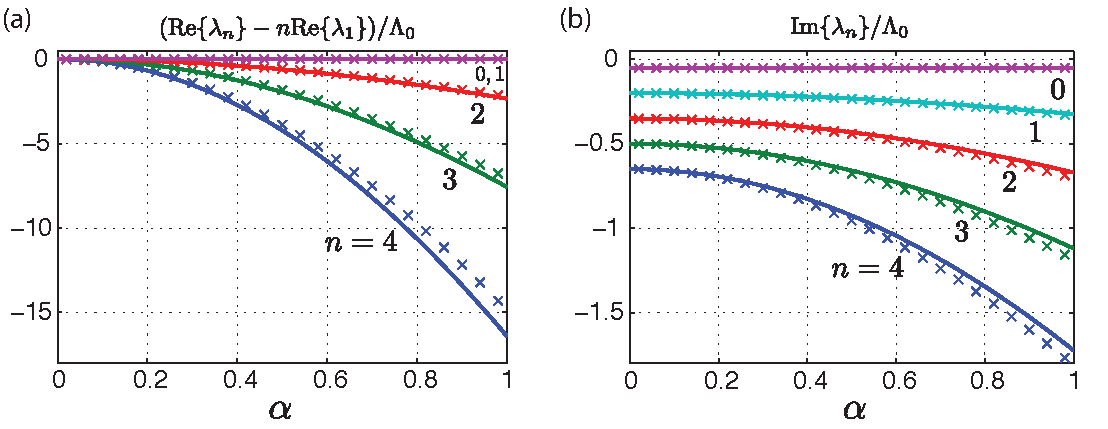
\includegraphics[width=1\textwidth]{./figs_Stannigel2012/Figure_suppl.pdf}
\caption
[Comparison of effective and exact description]
{Comparison of the effective analytic description
(Eqs.\,\eqref{eq:analytics}, lines) with exact eigenvalues of the Hamiltonian in
Eq.\,\eqref{eq:Hfull} (crosses) for different cavity field amplitudes $\alpha$.
All results are normalized to the scale
$\Lambda_0=g_0^4/(16\abs{\Delta_s}\delta^2)$ of the non-linearity.
(a) Deviation of the real parts of the eigenvalues from the result expected for
a linear oscillator, such that the splitting of the curves indicates an
effective non-linearity.
(b) Imaginary parts of the eigenvalues corresponding to decays. In both plots we
used the parameters $\Delta_s/g_0=-1$, $\delta/g_0=5$, $\kappa/g_0=2.5\times
10^{-2}$, $\gamma_m/g_0=2.5\times 10^{-4}$ and $N_{\rm th}=1$.}
\label{fig:numerics}
\end{figure}


To assess the validity of the effective phonon ME we now compare our result with
the dynamics of the full OMS.  Since we are mainly interested in the relation
between the phonon non-linearity and the corresponding dephasing and decay
rates, it is sufficient to evaluate the spectrum of the non-Hermitian
Hamiltonian, which  for the full model it is given by
\begin{equation}
\label{eq:Hfull}
\tilde H_{\rm full}=  H_{\rm lin}+ H_g - i\kappa c_s^\dag c_s - i\kappa
c_a^\dag c_a
 -i\frac{\gamma}{2} (N_{\rm th}+1) b^\dag b  -i\frac{\gamma}{2} N_{\rm th} b
b^\dag.
\end{equation}
In Fig.~\ref{fig:numerics} we plot the real and imaginary parts of the lowest
eigenvalues $\lambda_n$ of $\tilde H_{\rm full}$, which correspond to the lowest
number states $|n\rangle$ of the $B$ mode.
From the effective phonon model given in Eq.~\eqref{eq:SM_EffectiveME} and
\eqref{eq:SM_EffectiveME_corr} we obtain the approximate analytic results
\begin{subequations}
\label{eq:analytics}
\begin{equation}
{\rm Re} \{ \lambda_n\}= n \tilde \omega_m + n^2 \Lambda(n),
\end{equation}  
and
\begin{equation}
|{\rm Im} \{ \lambda_n\}|=\frac{\gamma}{2} N_{\rm th} + n \left(
\frac{\gamma}{2} (2N_{\rm th}+1) +\frac{\gamma^\prime}{2}\right) +n^2
\Gamma_\phi(n).
\end{equation}
\end{subequations}
We see a good agreement between these results for the effective model and the
exact numerics, both for the real and imaginary parts. Although there are some
deviations due to higher-order effects, the effective non-linear splitting
(Fig.~\ref{fig:numerics}(a)) is much larger than the induced decoherence
(Fig.~\ref{fig:numerics}(b)), as is expected for the chosen parameters. Hence,
we conclude that the effective model accurately describes the dynamics of the
mechanical resonator, and that the effective phonon non-linearity may serve as a
basis for gate operations as discussed in the main text and in the following
section.


\section{Phonon-phonon interactions} 

The derivation of the effective phonon nonlinearity, as outlined above for a
single resonator, can be easily adapted to two resonators as discussed in the
main text.
In this case we have 
\begin{equation}
H_0=  \sum_{i=1,2} \omega^i_m b_i^\dag b_i - \Delta_s c_s^\dag c_s - \Delta_a 
c_a^\dag c_a,
\end{equation}
and
\begin{equation}
H_g= \frac{g_0}{2} \left[c_a c_s^\dag (b^\dag_1-b_2^\dag) +    c_a^\dag c_s 
(b_1-b_2)\right].
\end{equation}
After changing into the displaced representation to eliminate the driving field
we obtain the linearized Hamiltonian
\begin{equation}
H_{\rm lin}�=  H_0  + \sqrt{2}\left( G(t)  c_a b_a^\dag + G^*(t) c_a^\dag
b_a\right),
\end{equation} 
where $b_a=(b_1-b_2)/\sqrt{2}$ and $G(t)=g_0\alpha(t)/2$.
For similar mechanical frequencies $\omega_m^1\simeq \omega_m^2=\omega_m$ the
symmetric resonator mode is decoupled and we can simply repeat the analysis from
above by identifying $b\equiv b_a$ and replacing $g_0$ by $\sqrt{2}g_0$.

For arbitrary $\omega_i$, we write the linear part of the Hamiltonian in its
diagonal form
\begin{equation}\label{eq:Hlin2}
H_{\rm lin}�=  - \Delta_s c_s^\dag c_s -  \tilde \Delta_a  C^\dag C + \tilde
\omega_1 B_1^\dag B_1 + \tilde \omega_2 B_2^\dag B_2.
\end{equation} 
As in the single-resonator case the $c_s$ mode is unaffected,  but the $c_a$
mode now couples to both $b_1$ and $b_2$.  The resulting hybridized modes $C$,
$B_\pm$ depend on the choice of parameters $\omega_m^{1,2}, \Delta_a$ and $G$.
For the case of interest, i.e. for a symmetric detuning
$\omega_m^{1,2}=-\Delta_a \mp \delta$, we obtain
\begin{eqnarray}
C&=& \cos(2\Theta) c_a -  \sin(2\Theta)(B_1 + B_2)/\sqrt{2},\\
B_1&=& \cos^2(\Theta) b_1 + \sin(2\Theta) c_a/\sqrt{2} -  \sin^2(\Theta)b_2,\\
B_2&=& \cos^2(\Theta) b_2 + \sin(2\Theta) c_a/\sqrt{2} -  \sin^2(\Theta)b_1,
\end{eqnarray} 
where $\tan(2\Theta)=-\sqrt{2} |G|/\delta$. Therefore, for small $\Theta$ the
modes $B_{1,2}$ correspond to the original mechanical resonator modes $b_{1,2}$
and $\tilde \omega_i\approx \omega_m^{i}$.

As above, we can now re-express the dissipation and the non-linear coupling
$H_g$ in terms of $C$ and $B_\pm$. The modified mechanical dissipation terms are
given
\begin{equation}
\tilde{\mathcal{L}}_\gamma =  \sum_{i=1,2}  \frac{\gamma}{2}�\cos^2(2\Theta)
\mathcal{D}_{\rm th}[B_i] + \frac{\kappa}{2} \sin^2(2\Theta) \mathcal{D}[B_i],
\end{equation}
and for small $\Theta$ the optical decay rate $\gamma^\prime =\kappa
\sin^2(2\Theta)$ is the same as given above and in the main text.
Using the decomposition of the non-linear coupling as done in
Eq.~\eqref{eq:SM_HgDecomp},  we obtain
\begin{equation}
H_g^{(1)}= \frac{g_0}{\sqrt{8} }\sin(2\Theta)   \left( c_s+c_s^\dag\right)
\left(B_1^\dag B_1 - B^\dag_2 B_2\right),
\end{equation} 
the contribution $H_g^{(2)}$ vanishes and 
\begin{equation}
H_g^{\prime}= \frac{g_0}{2  }\cos(2\Theta)   \left( C c_s^\dag
(B_1^\dag-B_2^\dag) + {\rm H.c.}  \right).
\end{equation}
We see that the structure and also the relative frequency scales are identical
to the corresponding terms discussed for the single resonator above. Therefore,
under the same conditions we can eliminate the cavity mode and  obtain the
effective phonon master equation
\begin{equation}
\begin{split}
\dot \rho_m =& -i\left[\sum_i \tilde \omega_i B_i^\dag B_i + \Lambda (B_1^\dag
B_1-B_2^\dag B_2)^2 �, \rho_m \right]  \\
&+ \Gamma_\phi \mathcal{D}[(B_1^\dag B_1-B_2^\dag B_2)]\rho_m   +
\tilde{\mathcal{L}}_\gamma \rho_m.
\end{split} 
\end{equation}
 For small $\Theta$ this equation reduces to ME  (8) in the main text and
 higher-order corrections can be included in the same way as discussed for the
 single resonator case.




% bibliography:
% if it does not compile automatically, move it out of the \ssp brackets,
% compile, then move it back
{\ssp % single-spacing
\bibliography{bibs}
}


\end{document}
